\documentclass[aspectratio=43]{beamer}

% Theme and color scheme
\usetheme{Madrid}
\usecolortheme{default}

% Packages
\usepackage[utf8]{inputenc}
\usepackage[T1]{fontenc}
\usepackage{graphicx}
\usepackage{amsmath}
\usepackage{amsfonts}
\usepackage{amssymb}
\usepackage{hyperref}
\usepackage{multicol}
\usepackage{tikz}
\usepackage{xcolor}
\usepackage{colortbl}
\usepackage{tabularx}
\usepackage{booktabs}
\usepackage{adjustbox}
\usepackage{subfig}

% Configure Beamer footnotes for citations
\setbeamerfont{footnote}{size=\scriptsize}
\setbeamertemplate{footnote}{%
  \parindent 1em\noindent%
  \raggedright
  \hbox to 1.8em{\hfil\insertfootnotemark}\insertfootnotetext\par%
}

% Configure Beamer footnotes for citations
\setbeamerfont{footnote}{size=\tiny}
\setbeamertemplate{footnote}{%
  \parindent 1em\noindent%
  \raggedright
  \hbox to 1.8em{\hfil\insertfootnotemark}\insertfootnotetext\par%
}

% Citation counter for each slide
\newcounter{slidecite}
\makeatletter
\newcommand{\resetcitecounter}{\setcounter{slidecite}{0}\setcounter{footnote}{0}}
% Reset counter at the beginning of each frame
\BeforeBeginEnvironment{frame}{\resetcitecounter}

% Force footnote numbering to use only Arabic numerals (no letters)
\renewcommand{\thefootnote}{\arabic{footnote}}
\renewcommand{\thempfootnote}{\arabic{mpfootnote}}
\makeatother

% Define citation texts as commands for reuse
\newcommand{\citeDavid}{David et al. Plant detection and counting from high-resolution RGB images acquired from UAVs. \textit{bioRxiv}, 2021}
\newcommand{\citeLiu}{Liu et al. IntegrateNet: A deep learning network for maize stand counting from UAV imagery. \textit{IEEE Geosci. Remote Sens. Lett.}, 19:6512605, 2022}
\newcommand{\citeMaizeSeeding}{Maize\_seeding dataset. \url{https://universe.roboflow.com/objectdetection-hytat/maize\_seeding}}
\newcommand{\citeMaizeSeedling}{Maize-seedling-detection dataset. \url{https://universe.roboflow.com/fyxdds-icloud-com/maize-seedling-detection}}
\newcommand{\citeFAO}{FAO. \textit{Agricultural Production Statistics 2010--2023}. FAOSTAT, Rome, Italy, 2024}
\newcommand{\citeMeier}{Meier et al. The BBCH system to coding the phenological growth stages of plants. \textit{J. Für Kult.}, 61:41--52, 2009}
\newcommand{\citeGarcia}{García-Martínez et al. Digital count of corn plants using UAVs and cross correlation. \textit{Agronomy}, 10:469, 2020}
\newcommand{\citeLeCun}{LeCun et al. Deep learning. \textit{Nature}, 521:436--444, 2015}
\newcommand{\citeFasterRCNN}{Faster R-CNN: Towards real-time object detection with region proposal networks}
\newcommand{\citeVaswani}{Vaswani et al. Attention is all you need. \textit{NIPS}, 2017}
\newcommand{\citeCarion}{Carion et al. End-to-end object detection with transformers. \textit{arXiv:2005.12872}, 2020}
\newcommand{\citeRekavandi}{Rekavandi et al. Transformers in small object detection: A benchmark and survey. \textit{arXiv:2309.04902}, 2023}
\newcommand{\citeZong}{Zong et al. DETRs with collaborative hybrid assignments training. \textit{ICCV}, 2023}
\newcommand{\citeBadgujar}{Badgujar et al. Agricultural object detection with YOLO algorithm. \textit{Comput. Electron. Agric.}, 223:109090, 2024}
\newcommand{\citeZhao}{Zhao et al. DETRs beat YOLOs on real-time object detection. \textit{arXiv:2304.08069}, 2024}
\newcommand{\citeBansal}{Bansal et al. Zero-shot object detection. \textit{ECCV}, 2018}
\newcommand{\citeHuang}{Huang et al. Survey on self-supervised few-shot learning, 2022}
\newcommand{\citeAndvaag}{Andvaag et al. Counting canola: Toward generalizable aerial plant detection. \textit{Plant Phenomics}, 6:0268, 2024}
\newcommand{\citeBarreto}{Barreto et al. Automatic UAV-based counting of seedlings. \textit{Comput. Electron. Agric.}, 191:106493, 2021}
\newcommand{\citeJiang}{Jiang et al. Deep seedling: Deep convolutional network, 2019}
\newcommand{\citeSun}{Sun et al. Revisiting unreasonable effectiveness of data in deep learning. \textit{arXiv:1707.02968}, 2017}
\newcommand{\citeAlhazmi}{Alhazmi et al. Effects of annotation quality on model performance. \textit{ICAIIC}, 2021}
\newcommand{\citeNguyen}{Nguyen et al. An evaluation of deep learning methods for small object detection. \textit{JECE}, 2020}
\newcommand{\citeBrigato}{Brigato et al. Close look at deep learning, 2020}
\newcommand{\citeDu}{Du et al. SpineNet: Learning scale-permuted backbone. \textit{CVPR}, 2020}
\newcommand{\citeRoggiolani}{Roggiolani et al. Domain-specific pre-training, 2023}
\newcommand{\citeShorten}{Shorten et al. A survey on image data augmentation for deep learning. \textit{J. Big Data}, 6:60, 2019}
\newcommand{\citeTan}{Tan et al. EfficientDet: Scalable efficient object detection, 2020}
\newcommand{\citeZhang}{Zhang et al. Comparison of YOLO-based sorghum detection, 2025}
\newcommand{\citePP}{PP1/333 (1) Adoption of Digital Technology for Data Generation for the Efficacy Evaluation of Plant Protection Products. \textit{EPPO Bull.}, 55:14--19, 2025}
\newcommand{\citeKraus}{Kraus, K. Photogrammetry: Geometry from Images and Laser Scans. De Gruyter: Berlin, Germany, 2011}
\newcommand{\citePugh}{Pugh et al. Comparison of image georeferencing strategies for agricultural applications of small unoccupied aircraft systems. \textit{Plant Phenome J.}, 4:e20026, 2021}
\newcommand{\citeHabib}{Habib et al. Automated Ortho-Rectification of UAV-Based Hyperspectral Data over an Agricultural Field Using Frame RGB Imagery. \textit{Remote Sens.}, 8:796, 2016}
\newcommand{\citeFarjon}{Farjon et al. Deep-learning-based counting methods, datasets, and applications in agriculture: A review. \textit{Precis. Agric.}, 24:1683--1711, 2023}
\newcommand{\citeVelumani}{Velumani et al. Estimates of Maize Plant Density from UAV RGB Images Using Faster-RCNN Detection Model. \textit{Plant Phenomics}, 2021:9824843, 2021}
\newcommand{\citeZou}{Zou et al. Maize Tassels Detection: A Benchmark of the State of the Art. \textit{Plant Methods}, 16:108, 2020}
\newcommand{\citeTorres}{Torres-Sánchez et al. Early Detection of Broad-Leaved and Grass Weeds in Wide Row Crops Using Artificial Neural Networks and UAV Imagery. \textit{Agronomy}, 11:749, 2021}
\newcommand{\citeLinCOCO}{Lin et al. Microsoft COCO: Common Objects in Context. \textit{arXiv}, arXiv:1405.0312, 2015}
\newcommand{\citeDosovitskiy}{Dosovitskiy et al. An Image Is Worth 16x16 Words: Transformers for Image Recognition at Scale. \textit{arXiv}, arXiv:2010.11929, 2021}
\newcommand{\citeKhan}{Khan et al. A Survey of the Vision Transformers and Their CNN-transformer Based Variants. \textit{Artif. Intell. Rev.}, 56:2917--2970, 2023}
\newcommand{\citeKhanam}{Khanam \& Hussain. YOLOv11: An Overview of the Key Architectural Enhancements. \textit{arXiv}, arXiv:2410.17725, 2024}
\newcommand{\citeLiMeta}{Li et al. Meta-SGD: Learning to Learn Quickly for Few-Shot Learning. \textit{arXiv}, arXiv:1707.09835, 2017}
\newcommand{\citeKang}{Kang et al. Few-shot Object Detection via Feature Reweighting. \textit{arXiv}, arXiv:1812.01866, 2019}
\newcommand{\citeMinderer}{Minderer et al. Scaling Open-Vocabulary Object Detection. \textit{Adv. Neural Inf. Process. Syst.}, 36:72983--73007, 2023}
\newcommand{\citeLiuGrounding}{Liu et al. Grounding DINO: Marrying DINO with Grounded Pre-training for Open-Set Object Detection. \textit{ECCV}, 2024}
\newcommand{\citeKarami}{Karami et al. Automatic Plant Counting and Location Based on a Few-Shot Learning Technique. \textit{IEEE J. Sel. Top. Appl. Earth Obs. Remote Sens.}, 13:5872--5886, 2020}
\newcommand{\citeWang}{Wang et al. Advancing Image Recognition: Towards Lightweight Few-shot Learning Model for Maize Seedling Detection. \textit{SCIS}, 2024}
\newcommand{\citeKitano}{Kitano et al. Corn Plant Counting Using Deep Learning and UAV Images. \textit{IEEE Geosci. Remote Sens. Lett.}, 16:1--5, 2019}
\newcommand{\citeHestness}{Hestness et al. Deep Learning Scaling Is Predictable, Empirically. \textit{arXiv}, arXiv:1712.00409, 2017}
\newcommand{\citeMahmood}{Mahmood et al. How Much More Data Do I Need? Estimating Requirements for Downstream Tasks. \textit{CVPR}, 2022}
\newcommand{\citeBumbacaDataset}{Bumbaca, Samuele. ‘The Original Dataset for the Paper "on the Minimum Data Set Requirements for Fine-tuning an Object Detector for Arable Crop Plant Counting: A Case Study on Maize Seedlings"’. Zenodo, 17 April 2025. https://doi.org/10.5281/zenodo.15235602.}
\newcommand{\citeFu}{Fu et al. Cross-Domain Few-Shot Object Detection via Enhanced Open-Set Object Detector. \textit{arXiv}, arXiv:2402.03094, 2024}
\newcommand{\citeTerven}{Terven et al. A Comprehensive Review of YOLO Architectures in Computer Vision: From YOLOv1 to YOLOv8 and YOLO-NAS. \textit{Mach. Learn. Knowl. Extr.}, 2023}
\newcommand{\citeJocher}{Jocher, Glenn; Qiu, Jiarui; Chaurasia, Anil. GitHub Ultralytics YOLO.  2023. Available online: \url{https://github.com/ultralytics/ultralytics}}

% Phytotoxicity scoring citations
\newcommand{\citeEPPODigital}{EPPO. PP 1/333(1) - Adoption of Digital Technology for Data Generation for the Efficacy Evaluation of Plant Protection Products. \textit{EPPO Bull.}, 55:14--19, 2025}
\newcommand{\citeEPPODesign}{EPPO. PP 1/135(2) - Design and analysis of efficacy evaluation trials. \textit{EPPO Bull.}, 42:367--381, 2014}
\newcommand{\citeChiangBias}{Chiang, K.-S.; et al. Effects of rater bias and assessment method on disease severity estimation. \textit{Plant Dis.}, 100:2530--2538, 2016}
\newcommand{\citeChiangQuantitative}{Chiang, K.-S.; et al. Understanding the ramifications of quantitative ordinal-scale measures. \textit{Plant Dis.}, 106:1051--1063, 2022}
\newcommand{\citeStevens}{Stevens, S.S. On the Theory of Scales of Measurement. \textit{Science}, 103:677--680, 1946}
\newcommand{\citeAgresti}{Agresti, A. Analysis of Ordinal Categorical Data. 2nd ed.; John Wiley \& Sons: Hoboken, NJ, USA, 2010}
\newcommand{\citeMahleinDetection}{Mahlein, A.-K. Plant disease detection and diagnosis by imaging sensors. \textit{Annu. Rev. Phytopathol.}, 54:373--393, 2016}
\newcommand{\citeMahleinHyperspectral}{Mahlein, A.-K.; et al. Hyperspectral sensors and imaging technologies in phytopathometry. \textit{Annu. Rev. Phytopathol.}, 56:535--558, 2018}
\newcommand{\citeGates}{Gates, D.M.; et al. Spectral properties of plants. \textit{Appl. Opt.}, 4:11--20, 1965}
\newcommand{\citeCarter}{Carter, G.A.; Knapp, A.K. Leaf optical properties in higher plants. \textit{Oecologia}, 128:442--452, 2001}
\newcommand{\citeGhosal}{Ghosal, S.; et al. An explainable deep machine vision framework for plant stress phenotyping. \textit{Proc. Natl. Acad. Sci. USA}, 115:4613--4618, 2018}
\newcommand{\citeGomezZamanillo}{Gómez-Zamanillo, A.; et al. Damage assessment in soybean and redroot pigweed plants exposed to herbicides. \textit{Agronomy}, 13:2523, 2023}

% Anomaly detection citations
\newcommand{\citeSavaryGlobal}{Savary et al. The global burden of pathogens and pests on major food crops. \textit{Nat. Ecol. Evol.}, 3:430--439, 2019}
\newcommand{\citeMartinelliAdvanced}{Martinelli et al. Advanced methods of plant disease detection. \textit{Agron. Sustain. Dev.}, 35:1--25, 2015}
\newcommand{\citeBarbedoFactors}{Barbedo, J.G.A. Factors influencing the use of deep learning for plant disease recognition. \textit{Biosyst. Eng.}, 172:84--91, 2018}
\newcommand{\citeFerentinosDeep}{Ferentinos, K.P. Deep learning models for plant disease detection and diagnosis. \textit{Comput. Electron. Agric.}, 145:311--318, 2018}
\newcommand{\citeMohantyUsing}{Mohanty et al. Using deep learning for image-based plant disease detection. \textit{Front. Plant Sci.}, 7:1419, 2016}
\newcommand{\citeSinghEffective}{Singh et al. Effective plant disease diagnosis using robust CNN architectures. \textit{Plant Methods}, 20:15, 2024}
\newcommand{\citeVallabhajosyulaNovel}{Vallabhajosyula et al. Novel hierarchical framework for plant disease classification. \textit{Appl. Sci.}, 14:3721, 2024}
\newcommand{\citeRuffUnifying}{Ruff et al. A unifying review of deep and shallow anomaly detection. \textit{Proc. IEEE}, 109:756--795, 2021}
\newcommand{\citeChalapathyDeep}{Chalapathy \& Chawla. Deep learning for anomaly detection: A survey. \textit{arXiv:1901.03407}, 2019}
\newcommand{\citeKatafuchiImage}{Katafuchi et al. Image-based plant disease detection using deep learning. \textit{Plant Pathol.}, 70:1021--1032, 2021}
\newcommand{\citeBumbacaSupporting}{Bumbaca et al. Supporting screening of new plant protection products. \textit{Agronomy}, 14:306, 2024}
\newcommand{\citeTodaHow}{Toda \& Okura. How convolutional neural networks diagnose plant disease. \textit{Plant Methods}, 15:9, 2019}
\newcommand{\citeHughesOpen}{Hughes \& Salathé. An open access repository of images on plant health. \textit{arXiv:1511.08060}, 2015}
\newcommand{\citeThapaPlant}{Thapa et al. The Plant Pathology 2020 challenge dataset. \textit{arXiv:2004.11958}, 2020}
\newcommand{\citeBreunigLOF}{Breunig et al. LOF: identifying density-based local outliers. \textit{SIGMOD}, 2000}
\newcommand{\citeScholkopfEstimating}{Schölkopf et al. Estimating the support of a high-dimensional distribution. \textit{Neural Comput.}, 13:1443--1471, 2001}
\newcommand{\citeLiuIsolation}{Liu et al. Isolation forest. \textit{IEEE ICDM}, 2008}

% Custom footnote citation command - ensures numeric-only marks
\newcommand{\fcite}[1]{%
  \stepcounter{footnote}%
  \textsuperscript{\thefootnote}%
  \footnotetext[\value{footnote}]{#1}%
}

% Custom colors
\definecolor{lightblue}{RGB}{173,216,230}
\definecolor{lightgray}{RGB}{211,211,211}
\definecolor{uniblue}{RGB}{0,51,102}
\definecolor{highlight}{RGB}{255,153,0}

% Environmental gradient colors (define globally)
\definecolor{envlow}{RGB}{255,245,235}     % Light orange
\definecolor{envmed}{RGB}{253,174,97}      % Medium orange
\definecolor{envhigh}{RGB}{215,48,31}      % Dark red

% Set theme colors
\setbeamercolor{structure}{fg=uniblue}
\setbeamercolor{frametitle}{bg=white,fg=black}

% Custom headline: white background + thin uniblue line at the bottom
\setbeamertemplate{frametitle}{
  \nointerlineskip
  \begin{beamercolorbox}[wd=\paperwidth,ht=2.5ex,dp=1ex,left]{frametitle}
    \hspace*{2em} % Move text right
    \vspace*{-1.5ex}\strut\insertframetitle\strut
  \end{beamercolorbox}
  \hspace*{-2em} % Move line right
  {\color{uniblue}\rule{\paperwidth}{0.7mm}}
}

% Remove navigation symbols
\setbeamertemplate{navigation symbols}{}

% Remove footline
\setbeamertemplate{footline}{}

% Custom title page
\setbeamertemplate{title page}{
    \begin{picture}(0,0)
        \put(25,-220){\includegraphics[width=0.8\paperwidth]{Imgs/Loghi.png}}
    \end{picture}
    \vfill
    \centering
    \begin{beamercolorbox}[sep=8pt,center]{title}
        \usebeamerfont{title}\inserttitle\par%
        \ifx\insertsubtitle\@empty%
        \else%
            \vskip0.25em%
            {\usebeamerfont{subtitle}\usebeamercolor[fg]{subtitle}\insertsubtitle\par}%
        \fi%
    \end{beamercolorbox}%
    \vskip1em\par
    \begin{beamercolorbox}[sep=8pt,center]{author}
        \usebeamerfont{author}\insertauthor
    \end{beamercolorbox}
    \begin{beamercolorbox}[sep=8pt,center]{institute}
        \usebeamerfont{institute}\insertinstitute
    \end{beamercolorbox}
    \begin{beamercolorbox}[sep=8pt,center]{date}
        \usebeamerfont{date}\insertdate
    \end{beamercolorbox}\vskip0.5em
    \vfill
}

% Document information
\title{Geomatic Techniques to Support Phytosanitary Products Tests whithin the EPPO Standard Framework}
\author{Samuele Bumbaca}
\institute{University of Turin}
\date{August 28, 2025}

\begin{document}

% Title slide
\begin{frame}
    \titlepage
\end{frame}

% Slide 2: The Traditional Approach to Agricultural Trials
\begin{frame}
    \frametitle{The Traditional Approach to Agricultural Trials}
    
    \begin{columns}
        \begin{column}{0.65\textwidth}
            \begin{center}
                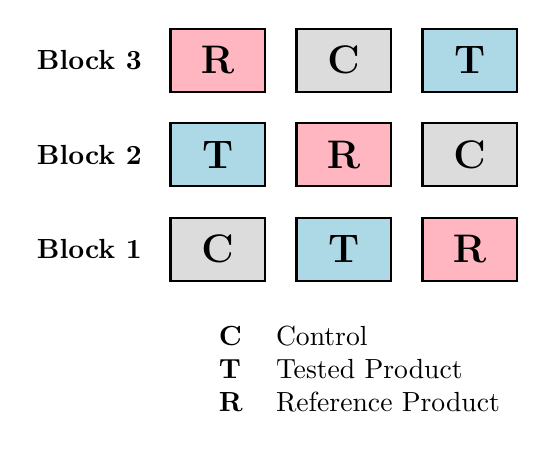
\begin{tikzpicture}[scale=0.8]
                    % Define colors for treatments
                    \definecolor{control}{RGB}{220,220,220}
                    \definecolor{tested}{RGB}{173,216,230}
                    \definecolor{reference}{RGB}{255,182,193}
                    
                    % Draw grid and plots
                    \foreach \row in {0,1,2} {
                        \foreach \col in {0,1,2} {
                            % Calculate position
                            \pgfmathsetmacro{\x}{\col*2}
                            \pgfmathsetmacro{\y}{\row*1.5}
                            
                            % Assign treatments (Latin square-like design)
                            \pgfmathsetmacro{\treatment}{int(mod(\col + \row, 3))}
                            \ifnum\treatment=0
                                \def\plotcolor{control}
                                \def\plotlabel{C}
                            \fi
                            \ifnum\treatment=1
                                \def\plotcolor{tested}
                                \def\plotlabel{T}
                            \fi
                            \ifnum\treatment=2
                                \def\plotcolor{reference}
                                \def\plotlabel{R}
                            \fi
                            
                            % Draw plot
                            \fill[\plotcolor] (\x,\y) rectangle (\x+1.5,\y+1);
                            \draw[black, thick] (\x,\y) rectangle (\x+1.5,\y+1);
                            \node at (\x+0.75,\y+0.5) {\Large\textbf{\plotlabel}};
                        }
                        % Block labels
                        \node[left] at (-0.3,\row*1.5+0.5) {\textbf{Block \pgfmathprint{int(\row+1)}}};
                    }
                    
                    % Legend
                    \node[below] at (3,-0.5) {
                        \begin{tabular}{ll}
                            \textbf{C} & Control \\
                            \textbf{T} & Tested Product \\
                            \textbf{R} & Reference Product
                        \end{tabular}
                    };
                \end{tikzpicture}
            \end{center}
        \end{column}
        
        \begin{column}{0.35\textwidth}
            \begin{block}{ANOVA Model:}
                \begin{equation*}
                    y_{ij} = \mu + \alpha_i + \beta_j + \varepsilon_{ij}
                \end{equation*}
                
                \small
                Where:
                \begin{itemize}
                    \item $y_{ij}$ = response
                    \item $\mu$ = overall mean
                    \item $\alpha_i$ = treatment effect
                    \item $\beta_j$ = block effect
                    \item $\varepsilon_{ij}$ = random error
                \end{itemize}
            \end{block}
            
            \begin{alertblock}{\tiny Note:}
                {\tiny This is the \textbf{additive model}. Modern approaches may include interaction terms: $\alpha_i \times \beta_j$}
            \end{alertblock}
        \end{column}
    \end{columns}
\end{frame}

% Slide 3: Key Assumptions of Traditional ANOVA
\begin{frame}
    \frametitle{Key Assumptions of Traditional ANOVA}
    
    \begin{block}{Statistical Assumptions:}
        \begin{itemize}
            \item \textbf{Randomization}: Treatments randomly assigned within blocks
            \item \textbf{Replication}: Each treatment appears in each block
            \item \textbf{Independence}: Observations are independent given the design
            \item \textbf{Homoscedasticity }: Equal variances across treatments
            \item \textbf{Normality}: Residuals follow normal distribution
        \end{itemize}
    \end{block}

    \begin{alertblock}{Consequences of Assumption Violations:}
        \begin{itemize}
            \item \textbf{Invalid conclusions of parametric tests}: Need for non-parametric tests leading to reduced statistical power
        \end{itemize}
    \end{alertblock}
    
    \vfill
    {\tiny
    \begin{flushleft}
        Based on R. A. Fisher, Statistical Methods for Research Workers, in S. Kotz \& N. L. Johnson (eds.), Breakthroughs in Statistics: Methodology and Distribution, pp. 66--70, Springer, New York, 1992.
    \end{flushleft}
    }
\end{frame}

% Slide 4: Right Blocking
\begin{frame}
    \frametitle{The Right Blocking: Capturing Environmental Variability}
    
    \begin{columns}
        \begin{column}{0.7\textwidth}
            \begin{center}
                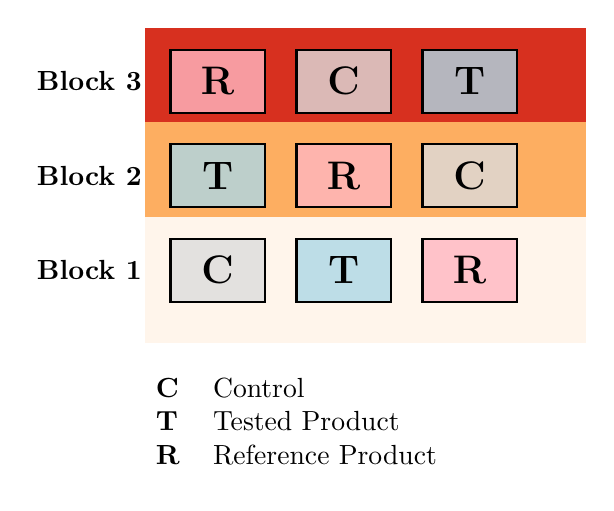
\begin{tikzpicture}[scale=0.8]
                    % Define colors for treatments
                    \definecolor{control}{RGB}{220,220,220}
                    \definecolor{tested}{RGB}{173,216,230}
                    \definecolor{reference}{RGB}{255,182,193}
                    
                    % Draw environmental variability strips (background)
                    \def\xoffset{0.1}
                    \def\yoffset{-0.15}
                    \fill[envlow] ({-0.5+\xoffset},{-0.5+\yoffset}) rectangle ({6.5+\xoffset},{1.5+\yoffset});
                    \fill[envmed] ({-0.5+\xoffset},{1.5+\yoffset}) rectangle ({6.5+\xoffset},{3+\yoffset});
                    \fill[envhigh] ({-0.5+\xoffset},{3+\yoffset}) rectangle ({6.5+\xoffset},{4.5+\yoffset});
                    
                    % Draw grid and plots
                    \foreach \row in {0,1,2} {
                        \foreach \col in {0,1,2} {
                            % Calculate position
                            \pgfmathsetmacro{\x}{\col*2}
                            \pgfmathsetmacro{\y}{\row*1.5}
                            
                            % Assign treatments (Latin square-like design)
                            \pgfmathsetmacro{\treatment}{int(mod(\col + \row, 3))}
                            \ifnum\treatment=0
                                \def\plotcolor{control}
                                \def\plotlabel{C}
                            \fi
                            \ifnum\treatment=1
                                \def\plotcolor{tested}
                                \def\plotlabel{T}
                            \fi
                            \ifnum\treatment=2
                                \def\plotcolor{reference}
                                \def\plotlabel{R}
                            \fi
                            
                            % Draw plot with some transparency to show environment
                            \fill[\plotcolor,opacity=0.8] (\x,\y) rectangle (\x+1.5,\y+1);
                            \draw[black, thick] (\x,\y) rectangle (\x+1.5,\y+1);
                            \node at (\x+0.75,\y+0.5) {\Large\textbf{\plotlabel}};
                        }
                        % Block labels
                        \node[left] at (-0.3,\row*1.5+0.5) {\textbf{Block \pgfmathprint{int(\row+1)}}};
                    }
                    
                    % Legend for treatments
                    \node[below] at (2,-1) {
                        \begin{tabular}{ll}
                            \textbf{C} & Control \\
                            \textbf{T} & Tested Product \\
                            \textbf{R} & Reference Product
                        \end{tabular}
                    };
                \end{tikzpicture}
            \end{center}
        \end{column}
        
        \begin{column}{0.3\textwidth}
            \begin{block}{\small Environmental Gradient:}
                \scriptsize
                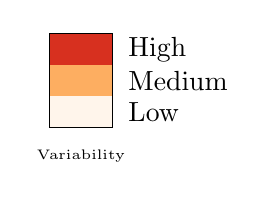
\begin{tikzpicture}[scale=0.8]
                    % Color scale bar
                    \fill[envlow] (0,0) rectangle (1,0.5);
                    \fill[envmed] (0,0.5) rectangle (1,1);
                    \fill[envhigh] (0,1) rectangle (1,1.5);
                    \draw[black] (0,0) rectangle (1,1.5);
                    
                    % Labels
                    \node[right] at (1.1,0.25) {Low};
                    \node[right] at (1.1,0.75) {Medium};
                    \node[right] at (1.1,1.25) {High};
                    \node[below] at (0.5,-0.2) {\tiny Variability};
                \end{tikzpicture}
            \end{block}
        \end{column}
    \end{columns}
    
    \begin{exampleblock}{\small Success of Blocking Strategy:}
        \begin{itemize}
            \scriptsize
            \item \textbf{Within-block homogeneity}: Treatments compared under similar conditions
            \item \textbf{Between-block heterogeneity}: Environmental gradient captured by block effects
        \end{itemize}
    \end{exampleblock}
\end{frame}

% Slide 5: The Wrong Blocking
\begin{frame}
    \frametitle{The Wrong Blocking: Assumption Violation}
    
    \begin{columns}
        \begin{column}{0.7\textwidth}
            \begin{center}
                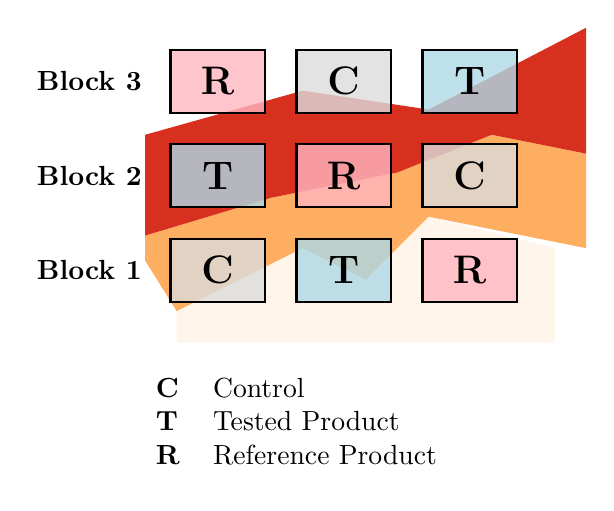
\begin{tikzpicture}[scale=0.8]
                    % Define colors for treatments
                    \definecolor{control}{RGB}{220,220,220}
                    \definecolor{tested}{RGB}{173,216,230}
                    \definecolor{reference}{RGB}{255,182,193}
                    
                    % Draw irregular environmental variability shapes (background)
                    \def\xoffset{0.1}
                    \def\yoffset{-0.15}
                    
                    % Irregular environmental patches that don't align with blocks
                    % Low variability (diagonal patches)
                    \fill[envlow] ({0+\xoffset},{0+\yoffset}) -- ({2+\xoffset},{1+\yoffset}) -- ({3+\xoffset},{0.5+\yoffset}) -- ({4+\xoffset},{1.5+\yoffset}) -- ({6+\xoffset},{1+\yoffset}) -- ({6+\xoffset},{-0.5+\yoffset}) -- ({0+\xoffset},{-0.5+\yoffset}) -- cycle;
                    
                    % Medium variability (curved patches)
                    \fill[envmed] ({-0.5+\xoffset},{1.2+\yoffset}) -- ({1.5+\xoffset},{1.8+\yoffset}) -- ({3.5+\xoffset},{2.2+\yoffset}) -- ({5+\xoffset},{2.8+\yoffset}) -- ({6.5+\xoffset},{2.5+\yoffset}) -- ({6.5+\xoffset},{1+\yoffset}) -- ({4+\xoffset},{1.5+\yoffset}) -- ({3+\xoffset},{0.5+\yoffset}) -- ({2+\xoffset},{1+\yoffset}) -- ({0+\xoffset},{0+\yoffset}) -- ({-0.5+\xoffset},{0.8+\yoffset}) -- cycle;
                    
                    % High variability (irregular top patches)
                    \fill[envhigh] ({-0.5+\xoffset},{2.8+\yoffset}) -- ({2+\xoffset},{3.5+\yoffset}) -- ({4+\xoffset},{3.2+\yoffset}) -- ({6.5+\xoffset},{4.5+\yoffset}) -- ({6.5+\xoffset},{2.5+\yoffset}) -- ({5+\xoffset},{2.8+\yoffset}) -- ({3.5+\xoffset},{2.2+\yoffset}) -- ({1.5+\xoffset},{1.8+\yoffset}) -- ({-0.5+\xoffset},{1.2+\yoffset}) -- cycle;
                    
                    % Draw grid and plots
                    \foreach \row in {0,1,2} {
                        \foreach \col in {0,1,2} {
                            % Calculate position
                            \pgfmathsetmacro{\x}{\col*2}
                            \pgfmathsetmacro{\y}{\row*1.5}
                            
                            % Assign treatments (Latin square-like design)
                            \pgfmathsetmacro{\treatment}{int(mod(\col + \row, 3))}
                            \ifnum\treatment=0
                                \def\plotcolor{control}
                                \def\plotlabel{C}
                            \fi
                            \ifnum\treatment=1
                                \def\plotcolor{tested}
                                \def\plotlabel{T}
                            \fi
                            \ifnum\treatment=2
                                \def\plotcolor{reference}
                                \def\plotlabel{R}
                            \fi
                            
                            % Draw plot with some transparency to show environment
                            \fill[\plotcolor,opacity=0.8] (\x,\y) rectangle (\x+1.5,\y+1);
                            \draw[black, thick] (\x,\y) rectangle (\x+1.5,\y+1);
                            \node at (\x+0.75,\y+0.5) {\Large\textbf{\plotlabel}};
                        }
                        % Block labels
                        \node[left] at (-0.3,\row*1.5+0.5) {\textbf{Block \pgfmathprint{int(\row+1)}}};
                    }
                    
                    % Legend for treatments
                    \node[below] at (2,-1) {
                        \begin{tabular}{ll}
                            \textbf{C} & Control \\
                            \textbf{T} & Tested Product \\
                            \textbf{R} & Reference Product
                        \end{tabular}
                    };
                \end{tikzpicture}
            \end{center}
        \end{column}
        
        \begin{column}{0.3\textwidth}
            \begin{block}{\small Environmental Gradient:}
                \scriptsize
                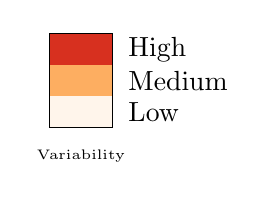
\begin{tikzpicture}[scale=0.8]
                    % Color scale bar
                    \fill[envlow] (0,0) rectangle (1,0.5);
                    \fill[envmed] (0,0.5) rectangle (1,1);
                    \fill[envhigh] (0,1) rectangle (1,1.5);
                    \draw[black] (0,0) rectangle (1,1.5);
                    
                    % Labels
                    \node[right] at (1.1,0.25) {Low};
                    \node[right] at (1.1,0.75) {Medium};
                    \node[right] at (1.1,1.25) {High};
                    \node[below] at (0.5,-0.2) {\tiny Variability};
                \end{tikzpicture}
            \end{block}
        \end{column}
    \end{columns}
    
    \begin{alertblock}{\small Heteroscedasticity Assumption Violation Problem:}
        \scriptsize
        \begin{itemize}
            \item \textbf{Blocks fail to capture environmental variability}: Treatments compared under different conditions
            \item \textbf{Invalid parametric test}: Residual variance differs across treatments
        \end{itemize}
    \end{alertblock}
\end{frame}

% Slide 6: The Problem
\begin{frame}
    \frametitle{Current Limitations in Statistics for Agricultural Trials}
    
    \begin{block}{Traditional Approach Issues:}
        \begin{itemize}
            \item \textbf{Human-dependent blocking}: Environmental variability assessment relies on experimenter experience
            \item \textbf{A priori identification}: Must identify variance sources BEFORE data collection
        \end{itemize}
    \end{block}
    
    \begin{alertblock}{The Challenge:}
        \textit{How can we capture environmental variability mathematically rather than through human judgment?}
    \end{alertblock}
\end{frame}

% Slide 7: Geostatistical Approach
\begin{frame}
    \frametitle{Geostatistical Approach: Spatial Linear Mixed Models}
    
    \begin{columns}
        \begin{column}{0.65\textwidth}
            \begin{center}
                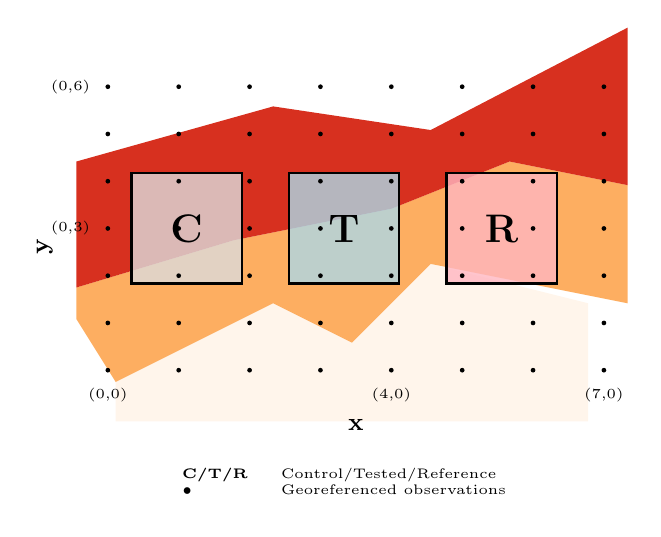
\begin{tikzpicture}[scale=1]
                    % Define colors for treatments
                    \definecolor{control}{RGB}{220,220,220}
                    \definecolor{tested}{RGB}{173,216,230}
                    \definecolor{reference}{RGB}{255,182,193}
                    
                    % Draw irregular environmental variability shapes (background)
                    \def\xoffset{0.1}
                    \def\yoffset{-0.15}
                    
                    % Same irregular environmental patches as slide 5
                    \fill[envlow] ({0+\xoffset},{0+\yoffset}) -- ({2+\xoffset},{1+\yoffset}) -- ({3+\xoffset},{0.5+\yoffset}) -- ({4+\xoffset},{1.5+\yoffset}) -- ({6+\xoffset},{1+\yoffset}) -- ({6+\xoffset},{-0.5+\yoffset}) -- ({0+\xoffset},{-0.5+\yoffset}) -- cycle;
                    
                    \fill[envmed] ({-0.5+\xoffset},{1.2+\yoffset}) -- ({1.5+\xoffset},{1.8+\yoffset}) -- ({3.5+\xoffset},{2.2+\yoffset}) -- ({5+\xoffset},{2.8+\yoffset}) -- ({6.5+\xoffset},{2.5+\yoffset}) -- ({6.5+\xoffset},{1+\yoffset}) -- ({4+\xoffset},{1.5+\yoffset}) -- ({3+\xoffset},{0.5+\yoffset}) -- ({2+\xoffset},{1+\yoffset}) -- ({0+\xoffset},{0+\yoffset}) -- ({-0.5+\xoffset},{0.8+\yoffset}) -- cycle;
                    
                    \fill[envhigh] ({-0.5+\xoffset},{2.8+\yoffset}) -- ({2+\xoffset},{3.5+\yoffset}) -- ({4+\xoffset},{3.2+\yoffset}) -- ({6.5+\xoffset},{4.5+\yoffset}) -- ({6.5+\xoffset},{2.5+\yoffset}) -- ({5+\xoffset},{2.8+\yoffset}) -- ({3.5+\xoffset},{2.2+\yoffset}) -- ({1.5+\xoffset},{1.8+\yoffset}) -- ({-0.5+\xoffset},{1.2+\yoffset}) -- cycle;
                    
                    % Add treatment rectangles in center Y of plot (larger rectangles)
                    \pgfmathsetmacro{\midY}{1.8}
                    \fill[color=control,opacity=0.8] (0.3,\midY-0.7) rectangle (1.7,\midY+0.7);
                    \draw[black, thick] (0.3,\midY-0.7) rectangle (1.7,\midY+0.7);
                    \node at (1,\midY) {\Large\textbf{C}};
                    
                    \fill[color=tested,opacity=0.8] (2.3,\midY-0.7) rectangle (3.7,\midY+0.7);
                    \draw[black, thick] (2.3,\midY-0.7) rectangle (3.7,\midY+0.7);
                    \node at (3,\midY) {\Large\textbf{T}};
                    
                    \fill[color=reference,opacity=0.8] (4.3,\midY-0.7) rectangle (5.7,\midY+0.7);
                    \draw[black, thick] (4.3,\midY-0.7) rectangle (5.7,\midY+0.7);
                    \node at (5,\midY) {\Large\textbf{R}};
                    
                    % Draw grid of observation points with coordinates (denser grid)
                    \foreach \row in {0,1,2,3,4,5,6} {
                        \foreach \col in {0,1,2,3,4,5,6,7} {
                            % Calculate position (adjusted for denser grid)
                            \pgfmathsetmacro{\x}{\col*0.9}
                            \pgfmathsetmacro{\y}{\row*0.6}
                            
                            % Draw observation point
                            \fill[black] (\x,\y) circle (0.03);
                            
                            % Add coordinate labels for some points (adjusted for new grid)
                            \ifnum\row=0
                                \ifnum\col=0
                                    \node[below, font=\tiny] at (\x,\y-0.1) {(0,0)};
                                \fi
                                \ifnum\col=4
                                    \node[below, font=\tiny] at (\x,\y-0.1) {(4,0)};
                                \fi
                                \ifnum\col=7
                                    \node[below, font=\tiny] at (\x,\y-0.1) {(7,0)};
                                \fi
                            \fi
                            \ifnum\col=0
                                \ifnum\row=3
                                    \node[left, font=\tiny] at (\x-0.1,\y) {(0,3)};
                                \fi
                                \ifnum\row=6
                                    \node[left, font=\tiny] at (\x-0.1,\y) {(0,6)};
                                \fi
                            \fi
                        }
                    }
                    
                    % Axis labels
                    \node[below, font=\small] at (3.15,-0.5) {\textbf{x}};
                    \node[left, font=\small, rotate=90] at (-0.8,1.8) {\textbf{y}};
                    
                    % Legend for treatments and spatial data
                    \node[below, font=\tiny] at (3,-1.1) {
                        \begin{tabular}{ll}
                            \textbf{C/T/R} & Control/Tested/Reference \\
                            \textbf{\(\bullet\)} & Georeferenced observations
                        \end{tabular}
                    };

                \end{tikzpicture}
            \end{center}
        \end{column}
        
        \begin{column}{0.35\textwidth}
            \begin{block}{\small Spatial LMM:}
                \begin{equation*}
                    y(s_i) = \mu + \alpha_j + f(s_i) + \varepsilon_i
                \end{equation*}
                
                \scriptsize
                Where:
                \begin{itemize}
                    \item $y(s_i)$ = response at $s_i$
                    \item $\mu$ = overall mean
                    \item $\alpha_j$ = treatment effect
                    \item $f(s_i)$ = spatial random field
                    \item $\varepsilon_i$ = error
                    \item $s_i = (x_i, y_i)$  = coordinates
                \end{itemize}
            \end{block}
            
        \end{column}
    \end{columns}
    
    \begin{exampleblock}{\scriptsize Benefits:}
        \tiny
        \begin{itemize}
            \item \textbf{No blocking}: Spatial correlation captures variability
            \item \textbf{Post-hoc}: No a priori variance identification
            \item \textbf{Homoscedasticity}: Assumption satisfied in more cases in respect blocking
        \end{itemize}
    \end{exampleblock}
\end{frame}

% Slide 8: Statistical Methods Comparison: Introduction
\begin{frame}
    \frametitle{Statistical Methods Comparison: Introduction}
    
    \begin{block}{Comparison Objective:}
        Evaluate the performance of \textbf{traditional RCBD} versus \textbf{spatial geostatistical methods} (SpATS) in capturing environmental variability and estimating treatment effects.
    \end{block}
    
    \begin{columns}
        \begin{column}{0.5\textwidth}
            \begin{exampleblock}{Synthetic Dataset:}
                \begin{itemize}
                    \item \textbf{\small 54 observations}\small (6\ensuremath{\times}9 grid)
                    \item \textbf{\small 3 treatments}\small : Control (0 t/ha), Reference (0.5 t/ha), Test (1.0 t/ha)
                    \item \textbf{\small 3 blocks}\small (18 plots each)
                    \item \textbf{\small Environmental zones}\small : Low (-1.5 t/ha), Medium (0 t/ha), High (+1.5 t/ha)
                \end{itemize}
            \end{exampleblock}
        \end{column}
        
        \begin{column}{0.5\textwidth}
            \begin{alertblock}{Tested Models:}
                \begin{enumerate}
                    \item \textbf{RCBD Model}: Linear Mixed Model with random block effects
                    \begin{equation*}
                        y_{ij} = \mu + \alpha_i + \beta_j + \varepsilon_{ij}
                    \end{equation*}
                    
                    \item \textbf{SpATS Model}: Spatial model with PSANOVA splines
                    \begin{equation*}
                        y(s) = \mu + \alpha_i + f(s) + \varepsilon(s)
                    \end{equation*}
                \end{enumerate}
            \end{alertblock}
        \end{column}
    \end{columns}
    
    \vspace{0.3cm}
    \begin{center}
        \small Where: $\alpha_i$ = treatment effects, $\beta_j$ = block effects, $f(s)$ = spatial smooth function, $s$ = coordinates
    \end{center}
\end{frame}

% Slide 9: Statistical Methods Comparison: The Field Trial
\begin{frame} %TODO: modify the R script to include all the legends reported in the slide in beamer tex language
    \frametitle{Statistical Methods Comparison: The Field Trial Design}
    
    \begin{center}
        \includegraphics[width=0.95\textwidth]{Imgs/integrated_rcbd_spats_comparison_irregular.png}
    \end{center}
    
    \begin{block}{\small Legend Interpretation:}
        \begin{columns}
            \begin{column}{0.33\textwidth}
                \textbf{Background Raster:}
                \begin{itemize}
                    \scriptsize
                    \item Environmental spatial effects
                    \item Irregular zones: Low/Medium/High
                    \item White to orange to red gradient
                \end{itemize}
            \end{column}
            
            \begin{column}{0.33\textwidth}
                \textbf{Purple Contours:}
                \begin{itemize}
                    \scriptsize
                    \item SpATS estimated spatial effects
                    \item Smooth spline interpolation
                    \item Continuous spatial modeling
                \end{itemize}
            \end{column}
            
            \begin{column}{0.33\textwidth}
                \textbf{Plot Elements:}
                \begin{itemize}
                    \scriptsize
                    \item \textbf{Rectangles}: Treatment effect magnitude (colored borders)
                    \item \textbf{Letters}: C/T/R treatments
                    \item \textbf{Corn symbols}: Individual yield observations (sized by value)
                \end{itemize}
            \end{column}
        \end{columns}
    \end{block}
\end{frame}

% Slide 10: Statistical Methods Comparison: Results
\begin{frame}
    \frametitle{Statistical Methods Comparison: Results}
    
    \begin{columns}
        \begin{column}{0.5\textwidth}
            \begin{block}{\small Model Performance \scriptsize (Mean Absolute Errors tonn/ha):}
                \begin{table}[h]
                    \centering
                    \scriptsize
                    \begin{tabular}{lcc}
                        \hline
                        \textbf{Model} & \textbf{Treat. Error} & \textbf{Env. Error} \\
                        \hline
                        RCBD Model & 0.13 & 0.62 \\
                        SpATS Spatial & 0.03 & 0.45 \\
                        \hline
                    \end{tabular}
                \end{table}
            \end{block}
            
            \begin{exampleblock}{\small Treatment Effect Estimation (tonn/ha):}
                \begin{table}[h]
                    \centering
                    \scriptsize
                    \begin{tabular}{lccc}
                        \hline
                        \textbf{Treatment} & \textbf{True} & \textbf{RCBD} & \textbf{SpATS} \\
                        \hline
                        Control & 0.00 & 0.00 & 0.00 \\
                        Reference & 0.50 & 0.40 & 0.45 \\
                        Test & 1.0 & 0.69 & 0.94 \\
                        \hline
                    \end{tabular}
                \end{table}
            \end{exampleblock}
        \end{column}
        
        \begin{column}{0.5\textwidth}
            \begin{alertblock}{\small Key Findings:}
                \begin{itemize}
                    \footnotesize
                    \item \textbf{Both models satisfied assumptions}
                    \item \textbf{SpATS outperformed RCBD}:
                    \begin{itemize}
                        \scriptsize
                        \item 3.8\ensuremath{\times} better treatment effect estimation
                        \item 1.4\ensuremath{\times} better environmental effect estimation
                    \end{itemize}
                    \item \textbf{RCBD underestimated} by 20-31\%
                    \item \textbf{SpATS <6\% error}
                \end{itemize}
            \end{alertblock}
            
            \begin{block}{\small Implications:}
                \scriptsize
                Even when traditional RCBD meets statistical assumptions, \textbf{spatial modeling provides superior accuracy} in treatment effect estimation by properly accounting for environmental spatial variability.
            \end{block}
        \end{column}
    \end{columns}
\end{frame}

% Slide 11: Research Gap
\begin{frame}
    \frametitle{The Missing Link: Spatial Coordinates}
    
    \begin{columns}
        \begin{column}{0.5\textwidth}
            \begin{block}{Geostatistical Methods Advantages:}
                \begin{itemize}
                    \item[\textcolor{green}{\checkmark}] \textbf{Mathematical modeling} of environmental variability
                    \item[\textcolor{green}{\checkmark}] \textbf{Post-hoc analysis} - no need for prior knowledge of the environment variables and of their distribution
                    \item[\textcolor{green}{\checkmark}] \textbf{Superior performance} in handling spatial heterogeneity
                    \item[\textcolor{green}{\checkmark}] \textbf{EPPO recognized} approach \scriptsize (PP1/152(4) - Design and analysis of efficacy evaluation trials)
                \end{itemize}
            \end{block}
        \end{column}
        
        \begin{column}{0.5\textwidth}
            \begin{alertblock}{Current Barrier:}
                \begin{itemize}
                    \item[\textcolor{red}{\(\times\)}] \textbf{Requires spatially referenced observations}
                    \item[\textcolor{red}{\(\times\)}] \textbf{Traditional manual assessments lack coordinates}
                    \item[\textcolor{red}{\(\times\)}] \textbf{Implementation gap} in practical field trials
                \end{itemize}
            \end{alertblock}
        \end{column}
    \end{columns}
\end{frame}

% Slide 12: Research Question
\begin{frame}
    \frametitle{Central Research Question}
    
    \begin{exampleblock}{}
        \large
        \textbf{Can geomatics technologies provide spatially referenced observations that enable geostatistical analysis within EPPO-compliant Plant Protection Product trials?}
    \end{exampleblock}
    
    \vspace{1em}
    
    \begin{block}{Specific Objectives:}
        \begin{enumerate}
            \item Establish which geomatics technologies can be used to collect spatially referenced observations
            \item Demonstrate the feasibility of collect spatially referenced observations in compliant with EPPO standards
            \item Validate performance against traditional methods
            \item Provide practical implementation guidelines
        \end{enumerate}
    \end{block}
\end{frame}

% Slide 13: Geomatic Techniques
\begin{frame}
    \frametitle{\small Geomatic Technologies: Workflow for Spatially Referenced Observations}
    
    \begin{center}
        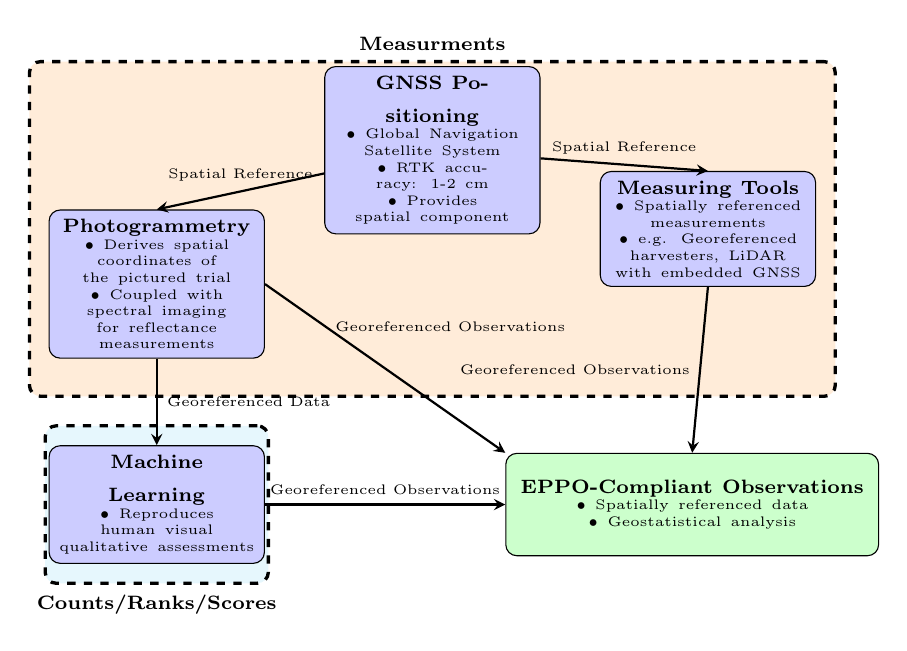
\begin{tikzpicture}[
            block/.style={rectangle, draw, fill=blue!20, text width=2.5cm, text centered, rounded corners, minimum height=1.3cm},
            arrow/.style={thick,->,>=stealth},
            groupbox/.style={rectangle, draw, rounded corners, very thick, dashed}
        ]
            
            % Background grouping rectangles
            % Light blue background for Visual assessments
            \node[groupbox, fill=cyan!10, text width=2.6cm, minimum height=2cm] (visual_group) at (-1,-2) {};
            \node[below] at (visual_group.south) {\scriptsize \textbf{Counts/Ranks/Scores}};
            
            % Light orange background for Continuous values
            \node[groupbox, fill=orange!15, text width=10cm, minimum height=4.25cm] (continuous_group) at (2.5,1.5) {};
            \node[above] at (continuous_group.north) {\scriptsize \textbf{Measurments}};
            
            % GNSS Block
            \node[block] (gnss) at (2.5,2.5) {
                \textbf{\scriptsize GNSS Positioning}\\
                \tiny
                $\bullet$ Global Navigation Satellite System\\
                $\bullet$ RTK accuracy: 1-2 cm\\
                $\bullet$ Provides spatial component\\
            };
            
            % Spectral Photogrammetry Block
            \node[block] (photogrammetry) at (-1,0.8) {
                \textbf{\scriptsize Photogrammetry}\\
                \tiny
                $\bullet$ Derives spatial coordinates of the pictured trial\\
                $\bullet$ Coupled with spectral imaging for reflectance measurements\\
            };
            
            % ML Inference Block
            \node[block] (ml) at (-1,-2) {
                \textbf{\scriptsize Machine Learning}\\
                \tiny
                $\bullet$ Reproduces human visual qualitative assessments\\
            };
            
            % Georeferenced Measuring Tools
            \node[block] (tools) at (6,1.5) {
                \textbf{\scriptsize Measuring Tools}\\
                \tiny
                $\bullet$ Spatially referenced measurements\\
                $\bullet$ e.g. Georeferenced harvesters, LiDAR with embedded GNSS\\
            };
            
            % Output Block
            \node[block, fill=green!20, text width=4.5cm] (output) at (5.8,-2) {
                \textbf{\scriptsize EPPO-Compliant Observations}\\
                \tiny
                $\bullet$ Spatially referenced data\\
                $\bullet$ Geostatistical analysis\\
            };

            % Arrows with proper syntax
            \draw[arrow] (gnss) -- (photogrammetry.north) node[midway,above] {\tiny Spatial Reference};
            \draw[arrow] (photogrammetry) -- (ml) node[midway,right] {\tiny Georeferenced Data};
            \draw[arrow] (ml.east) -- (output.west) node[midway,above] {\tiny Georeferenced Observations};
            \draw[arrow] (gnss) -- (tools.north) node[midway,above] {\tiny Spatial Reference};
            \draw[arrow] (tools.south) -- (output.north) node[midway,left] {\tiny Georeferenced Observations};
            \draw[arrow] (photogrammetry.east) -- (output.north west) node[near start,right] {\tiny Georeferenced Observations};
            % You can use [below], [above], [left], [right], [pos=0.5], [near start], [near end], [very near start], [very near end], [midway], [sloped], [bend left], [bend right], [out=angle], [in=angle], [loop], [shorten >=<length>], [shorten <=<length>], [looseness=<factor>], [distance=<length>], [swap], [auto], [anchor=<anchor>], [at end], [at start], [name path=<name>], [name intersections={of=<nameA> and <nameB>}], etc.
            % Example: \draw[->] (A) -- (B) node[midway, above] {Label};
        \end{tikzpicture}
    \end{center}

\end{frame}

% Slide 14: Georeferencing EPPO standard assessments
\begin{frame}
    \frametitle{Georeferencing EPPO Standard Assessments}
    
    \begin{table}[ht]
        \caption{\small EPPO's types of variables}
        \label{tab:data_types_slide}
        \centering
        \begin{tabular}{|l|c|c|c|}
        \hline
        \textbf{Type of Variable} & \textbf{Measurement} & \textbf{Ranking} & \textbf{Scoring} \\
        \hline
        \rowcolor{green!20} Continuous not limited & X & & \\
        \hline
        \rowcolor{green!20} Continuous limited & X & & \\
        \hline
        \rowcolor{yellow!20} Discrete & X & & \\
        \hline
        \rowcolor{red!20} Ordinal & & X & X \\
        \hline
        \rowcolor{red!20} Nominal & & & X \\
        \hline
        \rowcolor{red!20} Binary & & & X \\
        \hline
        \end{tabular}
        \end{table}
        
    \begin{flushleft}
        \hspace{1.5cm}{\tiny Summary from EPPO PP 1/152: Design and analysis of efficacy evaluation trials}
    \end{flushleft}

    \begin{block}{Current State of Georeferencing in Agricultural Trials:}
        \small Tool-based measurements (e.g., yield harvesters) can be easily georeferenced by integrating GNSS receivers on the tool. For visual assessments as counting, scoring or ranking, a method to transform georeferenced data to georeferenced observations is needed.
    \end{block}
\end{frame}

% Slide 15: ML Inference on Georeferenced Data
\begin{frame}
    \frametitle{Machine Learning Inference on Georeferenced Data}
    
    \begin{center}
        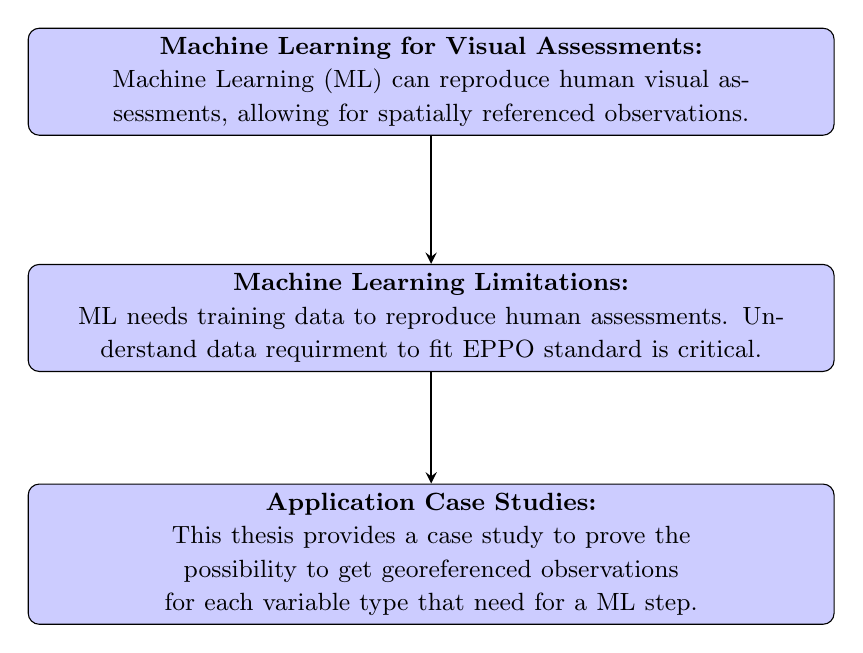
\begin{tikzpicture}[
            block/.style={rectangle, draw, fill=blue!20, text width=10cm, text centered, rounded corners, minimum height=1.3cm},
            arrow/.style={thick,->,>=stealth},
            groupbox/.style={rectangle, draw, rounded corners, very thick, dashed}
        ]
                        
            % First Block
            \node[block] (first) at (0,4) {
                \textbf{\small Machine Learning for Visual Assessments:}\\
            \small Machine Learning (ML) can reproduce human visual assessments, allowing for spatially referenced observations.        
            };
            % Second Block
            \node[block] (second) at (0,1) {
                \textbf{\small Machine Learning Limitations:}\\
            \small ML needs training data to reproduce human assessments. Understand data requirment to fit EPPO standard is critical.        
            };
            % Third Block
            \node[block] (third) at (0,-2) {
                \textbf{\small Application Case Studies:}\\
            \small This thesis provides a case study to prove the possibility to get georeferenced observations for each variable type that need for a ML step.         
            };

            % Arrows with proper syntax
            \draw[arrow] (first.south) -- (second.north);
            \draw[arrow] (second.south) -- (third.north);

        \end{tikzpicture}
    \end{center}
\end{frame}

% Slide 15: EPPO ML integration
\begin{frame}
    \frametitle{EPPO ML integration}
    
    \begin{block}{EPPO PP 1/333(1): Digital Technologies in PPP Trials}
        \small
        ML integrated assessments must meet the same quality standards as manual assessments and require validation through comparison with manual assessments (golden sample).
    \end{block}
    
    \begin{exampleblock}{\small Validation Benchmarks\footnote{\tiny Based on EPPO PP 1/333(1): Use of digital technologies in efficacy and selectivity trials}}
        \scriptsize
        \begin{itemize}
            \item \textbf{\large Continuous/Discrete}\large : $R^2 > 0.85$ (1:1 relationship)
            \item \textbf{\large Ordinal/Nominal}\large : Cohen's $\kappa > 0.7$
            \item \textbf{\large Binary}\large : Accuracy $> 0.85$
        \end{itemize}
    \end{exampleblock}
\end{frame}

% Slide 16: Georeferencing EPPO Standard Assessments: Case Studies
\begin{frame}
    \frametitle{Georeferencing Gap in EPPO Standard Assessments}
    \begin{table}[ht]
        \centering
        \begin{tabular}{|c|l|c|c|c|}
        \hline
        & \textbf{Type of Variable} & \textbf{Measurement} & \textbf{Ranking} & \textbf{Scoring} \\
        \hline
        \rowcolor{green!20} & Continuous not limited & X & & \\
        \hline
        \rowcolor{green!20} & Continuous limited & X & & \\
        \hline
        \rowcolor{yellow!20} $\rightarrow$ & Discrete & X & & \\
        \hline
        \rowcolor{red!20} $\rightarrow$ & Ordinal & & X & X \\
        \hline
        \rowcolor{red!20} $\rightarrow$ & Nominal & & & X \\
        \hline
        \rowcolor{red!20} $\rightarrow$ & Binary & & & X \\
        \hline
        \end{tabular}
    \end{table}
    \begin{block}{Case Studies:}
        \small This thesis aim to prove the reliability of georeferencing every EPPO standard assessmentEach case study addresses a specific variable type as defined in the EPPO standards
        \begin{itemize}
            \item \textbf{Discrete (Counts)} : Plant counting
            \item \textbf{Ordinal} : Phytotoxicity scoring
            \item \textbf{Nominal} and \textbf{Binary} : Disease detection 
        \end{itemize}
    \end{block}
\end{frame}

% PLANT COUNTING CASE STUDY

% Slide 17: Georeferencing Counts (Discrete Variable) 
\begin{frame}
    \frametitle{Georeferencing Counts (Discrete Variable)}
    \begin{table}[ht]
        \centering
        \begin{tabular}{|c|l|c|c|c|}
        \hline
        & \textbf{Type of Variable} & \textbf{Measurement} & \textbf{Ranking} & \textbf{Scoring} \\
        \hline
        \rowcolor{green!20} & Continuous not limited & X & & \\
        \hline
        \rowcolor{green!20} & Continuous limited & X & & \\
        \hline
        \rowcolor{yellow!20} $\rightarrow$ & Discrete & X & & \\
        \hline
        \rowcolor{red!20} & Ordinal & & X & X \\
        \hline
        \rowcolor{red!20} & Nominal & & & X \\
        \hline
        \rowcolor{red!20} & Binary & & & X \\
        \hline
        \end{tabular}
    \end{table}
    \begin{block}{Georeferencing Counts:}
        \small
        \begin{itemize}
            \item \textbf{Counts} are discrete variables required for measuring density of individuals (e.g. plant density in PP1/46 (3) - Wireworms).
            \item the \textbf{Case Study}: Counting plants from georeferenced photogrammetric orthomosaics by ML Object Detection. 
            \item this study is discussed in the scientific article \textbf{\scriptsize Bumbaca, S.; Borgogno-Mondino, E.C. On the Minimum Dataset Requirements for Fine-Tunining an Object Detector for Arable Crop Plant Counting: A Case Study on Maize Seedlings. Remote Sens. 2025, 17, 2190. DOI: 10.3390/rs1713219061}
        \end{itemize}
    \end{block}
\end{frame}

% Slide 18: Plant Counting Introduction - The Problem
\begin{frame}
    \frametitle{Arable Crop Plant Counting by Object Detection}
    
    \begin{block}{The Critical Need after EPPO Assessments:}
        \begin{itemize}
            \item Plant counting is \textbf{fundamental} also in precision agriculture and plant breeding
            \item Traditional manual counting is \textbf{time-consuming} and bring \textbf{human error} risks
            \item \textbf{Computer vision} offers a solution, but requires \textbf{dataset size and quality} characterization to prove the reliability for this task.
        \end{itemize}
    \end{block}
    
    \begin{exampleblock}{EPPO Benchmark Standards:}
        Coefficient of determination ($R^2$) $\geq$ 0.85 of ML method w.r.t. manual counting (no bias nor slope linear first order relation)
    \end{exampleblock}
    
    \begin{alertblock}{Research Gap:}
        \textit{What are the minimum dataset requirements to achieve this benchmark across different inference datasets?}
    \end{alertblock}
\end{frame}

% Slide 19: Georeferenced Orthomosaics
\begin{frame}
    \frametitle{Photogrammetric Orthomosaics for Plant Counting}
    
    \begin{block}{Advantages over other kind of data:}
        \begin{itemize}
            \item \textbf{Geographical coordinates}\small : Suitable for spatial analysis
            \item \textbf{Fixed scale and orientation images}\small : Eliminate perspective inconsistencies
            \item \textbf{Achievable High-resolution}\small : From low altitude nadiral overlapping images\fcite{\citeKraus}
        \end{itemize}
    \end{block}

    \includegraphics[width=1\textwidth]{Imgs/dataset_example.png}
\end{frame}

% Slide 20:
\begin{frame}
    \begin{alertblock}{Limitations:}
        \begin{itemize}
            \item \textbf{Occlusions}\small : Overlapping vegetation canopy issues \fcite{\citeHabib} -> Target crop and phenological stage selection
            \item \textbf{Georeferencing errors}\small : Due to low-quality/insufficient GNSS embedded systems or Ground Control Points (GCPs) \fcite{\citePugh} -> Hardware requirements
            \item \textbf{Computational demand}\small : Processing time constraints for large-area orthomosaics -> Not real-time suitable
        \end{itemize}
    \end{alertblock}
\end{frame}


% Slide 20: Plant Counting - Case Study Selection
\begin{frame}
    %\frametitle{Case Study: Maize Seedling Counting}
    
    \begin{block}{\small Plants Occlusion Solution: Maize Seedlings at BBCH 13-15 Stage}
        \small
        \begin{itemize}
            \item \textbf{\scriptsize Optimal detection conditions}\scriptsize : Regular planting pattern, minimal plant overlapping at BBCH 13-15 stage \fcite{\citeMeier}
            \item \textbf{\scriptsize Data availability}\scriptsize : Most represented plant in scientific \fcite{\citeDavid} \fcite{\citeLiu} and public datasets
            \item \textbf{\scriptsize Economic importance}\scriptsize : World's highest-production crop \fcite{\citeFAO}
            \item \textbf{\scriptsize Rappresentative crop}\scriptsize : Findings applicable to other row crops \fcite{\citeTorres} (e.g. Sunflower, Sugar beet)
        \end{itemize}
    \end{block}

    \begin{center}
        \includegraphics[width=0.4\textwidth]{Imgs/BBCH_Maize1315.png}
    \end{center}

\end{frame}

% Slide 21: Suitable Hardware and Picturing
\begin{frame}
    \begin{block}{\small Suitable Hardware and Photogrammetric Picturing}
        \small
        \begin{itemize}
            \item \textbf{UAV Platform}: Phantom 4 Pro v2.0 (DJI, Shenzhen, China)
            \item \textbf{Camera}: Default series RGB camera
            \item \textbf{Flight Altitude}: ~10 m above ground level
            \item \textbf{Original GSD}: 2.7 mm/pixel
            \item \textbf{GNSS Mode}: VRS-NRTK for GCP surveying
            \item \textbf{Bundle Adjustment Error}: 38 mm
            \item \textbf{Final Orthomosaic GSD}: 5 mm/pixel
            \item \textbf{Reference System}: WGS84/UTM 32 N
        \end{itemize}
    \end{block}
    
    \begin{block}{\small Key Processing Steps:}
        \small
        \begin{enumerate}
            \item Nadiral image capture with 70\%-80\% overlapping patterns
            \item Ground Control Points (GCPs) surveyed with high-precision GNSS
            \item Photogrammetric bundle adjustment and orthomosaic generation
            \item Georeferenced orthomosaic output ready for spatial analysis
        \end{enumerate}
    \end{block}
\end{frame}

% Slide 22: Plant Counting - Object Detection Paradigms
% COMMENTED OUT DUE TO EXCLUSION FROM THE PRESENTATION OF HC, FEW-SHOT AND ZERO-SHOT METHODS
%\begin{frame}
%    \frametitle{Plant Counting - Object Detection Paradigms}
%    The State-Of-The-Art (SOTA) methods to count plants by orthomosaics rely on object detectors. Historically, for most of the tasks, object detectors increased their performance in this order:
%    \begin{block}
%        \small
%        \begin{itemize}
%            \item \textbf{Traditional Methods}: Handcrafted features (hardcoded) - untill 1990s
%            \item \textbf{Machine Learning Approaches}: 1990s to 2010s
%            \item \textbf{Deep Learning Approaches}: Convolutional Neural Networks (CNNs) - 2010s to 2020s 
%            \item \textbf{Transformer Architectures}: Attention mechanisms introduction - 2020s
%            \item \textbf{Data-Efficient Methods}: Few-Shot and Zero-Shot Detection - Now
%        \end{itemize}
%    \end{block}
%\end{frame}

% Slide 23: Plant Counting - Classic Object Detection Methods
% COMMENTED OUT DUE TO EXCLUSION FROM THE PRESENTATION OF HC, FEW-SHOT AND ZERO-SHOT METHODS
%\begin{frame}
%    \frametitle{Plant Counting - Classic Object Detection Methods}
%    
%    \begin{block}{Handcrafted Methods (HC):}
%        \scriptsize
%        \begin{itemize}
%            \item \textbf{Traditional approach}: Still used in agricultural applications \fcite{\citeDavid} \fcite{\citeGarcia}
%            \item \textbf{Explicit programming}: Color thresholding, edge detection, morphological operations
%            \item \textbf{Advantages}: Domain expertise, interpretability, computational efficiency
%        \end{itemize}
%    \end{block}
%    \begin{center}
%        \includegraphics[width=1\textwidth]{Imgs/F2.large.jpg}
%    \end{center}
%\end{frame}

% Slide 24: Plant Counting - Classic Object Detection Methods
% MODIFIED DUE TO EXCLUSION FROM THE PRESENTATION OF HC, FEW-SHOT AND ZERO-SHOT METHODS
\begin{frame}
%    \frametitle{Plant Counting - Classic Object Detection Methods}
    \frametitle{Plant Counting - Object Detection Methods}
    \begin{columns}
        \begin{column}{0.5\textwidth}
            \begin{exampleblock}{Machine (Deep) Learning Approaches:}
                \scriptsize
                \textbf{Convolutional Neural Networks} \fcite{\citeLeCun}
                Grid-based convolutions
                \begin{itemize}
                    \item \textbf{Faster R-CNN} \fcite{\citeFasterRCNN}
                    \item \textbf{YOLO variants} for faster inference
                \end{itemize}
                
            \end{exampleblock}
        \end{column}
        
        \begin{column}{0.5\textwidth}
            \begin{exampleblock}{}
                \scriptsize
                \textbf{Transformer Architectures} \fcite{\citeVaswani}
                Image patches processing (attention-based)
                \begin{itemize}
                    \item \textbf{DETR} \fcite{\citeCarion}
                    \item \textbf{Hybrid approaches} with convolutions and attention
                \end{itemize}
                Superior with scarce data \fcite{\citeRekavandi}
            \end{exampleblock}
        \end{column}
    \end{columns}
    
    \begin{center}
        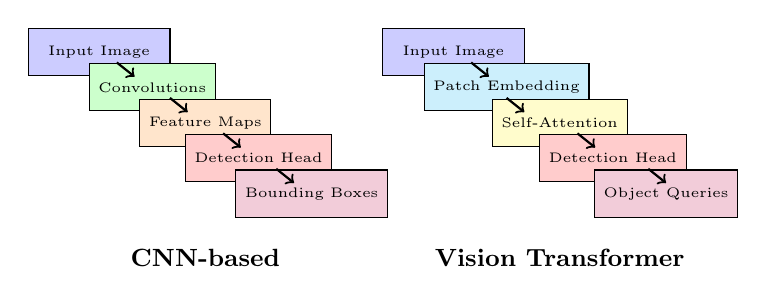
\begin{tikzpicture}[scale=0.45]
            % CNN Architecture (Left side) - Diagonal arrangement
            \node[draw, rectangle, fill=blue!20, minimum width=1.8cm, minimum height=0.6cm] at (-11, 2) {\tiny Input Image};
            
            % Conv layers (combined)
            \node[draw, rectangle, fill=green!20, minimum width=1.5cm, minimum height=0.6cm] at (-9.5, 1) {\tiny Convolutions};
            
            % Feature extraction
            \node[draw, rectangle, fill=orange!20, minimum width=1.5cm, minimum height=0.6cm] at (-8, 0) {\tiny Feature Maps};
            
            % Detection head
            \node[draw, rectangle, fill=red!20, minimum width=1.3cm, minimum height=0.6cm] at (-6.5, -1) {\tiny Detection Head};
            \node[draw, rectangle, fill=purple!20, minimum width=1.5cm, minimum height=0.6cm] at (-5, -2) {\tiny Bounding Boxes};
            
            % Arrows for CNN (diagonal flow)
            \draw[->, thick] (-10.5, 1.7) -- (-10, 1.3);
            \draw[->, thick] (-9, 0.7) -- (-8.5, 0.3);
            \draw[->, thick] (-7.5, -0.3) -- (-7, -0.7);
            \draw[->, thick] (-6, -1.3) -- (-5.5, -1.7);
            
            % Label for CNN
            \node[font=\small\bf] at (-8, -3.8) {CNN-based};
            
            % Vision Transformer Architecture (Right side) - Diagonal arrangement
            \node[draw, rectangle, fill=blue!20, minimum width=1.8cm, minimum height=0.6cm] at (-1, 2) {\tiny Input Image};
            
            % Patch embedding
            \node[draw, rectangle, fill=cyan!20, minimum width=1.5cm, minimum height=0.6cm] at (0.5, 1) {\tiny Patch Embedding};
            
            % Transformer blocks (simplified)
            \node[draw, rectangle, fill=yellow!20, minimum width=1.5cm, minimum height=0.6cm] at (2, 0) {\tiny Self-Attention};
            
            % Detection head
            \node[draw, rectangle, fill=red!20, minimum width=1.3cm, minimum height=0.6cm] at (3.5, -1) {\tiny Detection Head};
            \node[draw, rectangle, fill=purple!20, minimum width=1.5cm, minimum height=0.6cm] at (5, -2) {\tiny Object Queries};
            
            % Arrows for ViT (diagonal flow)
            \draw[->, thick] (-0.5, 1.7) -- (0, 1.3);
            \draw[->, thick] (0.5, 0.7) -- (1, 0.3);
            \draw[->, thick] (2.5, -0.3) -- (3, -0.7);
            \draw[->, thick] (4.5, -1.3) -- (5, -1.7);
            
            % Label for ViT
            \node[font=\small\bf] at (2, -3.8) {Vision Transformer};
            
            % Central dividing line (vertical)
            %\draw[dashed, gray, thick] (0, 2.5) -- (0, -3.2);
        \end{tikzpicture}
    \end{center}
\end{frame}

% Slide 25: Plant Counting - Data-Efficient Detection Methods
% COMMENTED OUT DUE TO EXCLUSION FROM THE PRESENTATION OF HC, FEW-SHOT AND ZERO-SHOT METHODS
%\begin{frame}
%    \frametitle{Plant Counting - Data-Efficient Detection Methods}
%    
%    \begin{columns}
%        \begin{column}{0.5\textwidth}
%            \begin{block}{Few-Shot Detection:}
%                \small
%                \begin{itemize}
%                    \item \textbf{Learning from minimal examples}: 1-30 annotated instances
%                    \item \textbf{Meta-learning} approach \fcite{\citeLiMeta}
%                    \item \textbf{Advantage}: Reduce annotation burden for new classes
%                    \item \textbf{Limited studies}: Only two for maize seedlings \fcite{\citeKarami} \fcite{\citeWang}
%                \end{itemize}
%            \end{block}
%        \end{column}
%        \begin{column}{0.5\textwidth}
%            \includegraphics[width=1\textwidth]{Imgs/fewshot.png}
%            \fcite{https://si-analytics.tistory.com/}
%        \end{column}
%    \end{columns}
%\end{frame}

% Slide 25: Plant Counting - Data-Efficient Detection Methods - Zero-Shot Detection
% COMMENTED OUT DUE TO EXCLUSION FROM THE PRESENTATION OF HC, FEW-SHOT AND ZERO-SHOT METHODS
%\begin{frame}
%    \frametitle{Plant Counting - Data-Efficient Detection Methods}
%    \begin{columns}
%        \begin{column}{0.5\textwidth}
%            \begin{block}{Zero-Shot Detection:}
%                \small
%                \begin{itemize}
%                    \item \textbf{No labeled examples}: Detect novel objects without training data
%                    \item \textbf{Semantic relationships}: Exploit contextual information \fcite{\citeBansal}
%                    \item \textbf{State-of-the-art}: OWLv2 \fcite{\citeMinderer}, Grounding DINO \fcite{\citeLiuGrounding}
%                    \item \textbf{Agricultural gap}: No studies for maize seedling counting
%                \end{itemize}
%            \end{block}
%        \end{column}
%        \begin{column}{0.5\textwidth}
%            \includegraphics[width=0.8\textwidth]{Imgs/OWL2v.png}
%            \fcite{\citeMinderer}
%        \end{column}
%    \end{columns}
%\end{frame}

% Slide 26: Plant Counting - Data Scarcity Challenge
% MODIFIED DUE TO EXCLUSION FROM THE PRESENTATION OF HC, FEW-SHOT AND ZERO-SHOT METHODS
\begin{frame}
    \frametitle{Plant Counting - Research Gap}
    \begin{alertblock}{Critical Research Gaps:}
        \begin{itemize}
            \item \textbf{Minimum dataset requirements} None of the studies taken into account systematically tested\fcite{\citeSun} the minimum dataset requirements for robust plant detectors (EPPO benchmark).
            \item \textbf{In-domain vs. out-of-distribution data} Despite some author already studied the impact\fcite{\citeDavid} \fcite{\citeAndvaag} none did it in a quantitative and systematic way.
%            \item \textbf{Architecture influence} Many studies compared different architectures, someone claiming few-shot performances \fcite{\citeWang} \fcite{\citeKarami}, but none systematically tested the minimum dataset capability and none tested the zero-shot possibility.
        \end{itemize}
    \end{alertblock}

\end{frame}

% Slide 27: Study Aim
\begin{frame}
    \frametitle{Study Aim}
    
    \begin{exampleblock}{Primary Objective:}
        Establish the \textbf{minimum dataset requirements} for accurate maize seedling detection (EPPO benchmark) in georeferenced orthomosaics across different object detection paradigms
    \end{exampleblock}
    
    \begin{block}{Key Definitions:}
        \small
        \begin{itemize}
            \item \textbf{Dataset size}: Amount of annotated images in training set
            \item \textbf{Dataset quality}: Accuracy of annotations (percentage of correct annotations relative to ground truth)
        \end{itemize}
    \end{block}
    
    \begin{block}{Specific Research Questions:}
        \small
        \begin{enumerate}
            \item How does training data source (in-domain vs. out-of-distribution) affect required dataset size and quality?
            \item Untill which extent different architectures affect training dataset requirements?
        \end{enumerate}
    \end{block}
\end{frame}

% Slide 28: Plant Counting - Material and Methods - The Systematic Approach
% COMMENTED OUT DUE TO EXCLUSION FROM THE PRESENTATION OF HC, FEW-SHOT AND ZERO-SHOT METHODS
\begin{frame}
    \frametitle{Plant Counting - Material and Methods - Research Methodology}
    \small
    \begin{itemize}
        \item \textbf{Objective}: Investigate minimum dataset size and quality for robust object detection
%        \item \textbf{Handcrafted Method}: Test Handcrafted (HC) algorithm performances on test dataset.
        \item \textbf{Classic Object Detectors requirements}:
            \begin{itemize}
                \item with out-of-distribution (OOD) training datasets.
                \item with in-domain (ID) training datasets.
            \end{itemize} 
%        \item \textbf{Data-efficient Methods}: 
%            \begin{itemize}
%                \item Test Few-Shot Detector requirements with ID training samples.
%                \item Test Zero-Shot Detector performances.
%            \end{itemize}
        \item \textbf{Empirical Modeling Approach}:
            \begin{itemize}
                \item Analyze the relationship between dataset size/quality and model performance
                \item Fit empirical functions to characterize this relationship
                \item Use fitted functions to predict performance with varying dataset size/quality
            \end{itemize}
    \end{itemize}
\end{frame}

% Slide 31: Plant Counting - Material and Methods - Dataset
\begin{frame}
    \frametitle{Plant Counting - Material and Methods - Dataset}
    
    \begin{block}{Dataset Classification:}
        \small
        \begin{itemize}
            \item \textbf{Out-of-Distribution (OOD)}: Training datasets from different sources than inference target
            \item \textbf{In-Domain (ID)}: Training datasets from same source/distribution as testing dataset
        \end{itemize}
    \end{block}
    
    \begin{columns}
        \begin{column}{0.5\textwidth}
            \begin{block}{OOD Scientific Datasets:}
                    \textbf{Source}: Scientific literature
            \end{block}
            
            \begin{block}{OOD Internet Datasets:}
                \textbf{Source}: Internet repositories
            \end{block}
        \end{column}
        
        \begin{column}{0.5\textwidth}
            \begin{block}{ID Datasets:}
                \textbf{Source}: Collected by the author
            \end{block}
            
            \begin{exampleblock}{Key Processing Parameters:}
                \scriptsize
                    All dataset preprocessed to get standard \textbf{tile size}: 224\ensuremath{\times}224 pixels (1.12\ensuremath{\times}1.12 m field coverage for georeferenced)
            \end{exampleblock}
        \end{column}
    \end{columns}
\end{frame}

% Slide 32: Plant Counting - Material and Methods - Dataset
\begin{frame}
    \scriptsize
    \frametitle{Plant Counting - Material and Methods - Datasets}
    \begin{table}[H]
        \begin{tabularx}{\textwidth}{llXX}
        \toprule
        \textbf{Dataset} & \textbf{Phenological Stage} & \textbf{Train Size} & \textbf{Test Size} \\
        \midrule
        \multicolumn{4}{l}{OOD Scientific} \\
        \hspace{0.5em}DavidEtAl.2021~\fcite{\citeDavid} & V3 & 182 tiles & N/A* \\
        \hspace{0.5em}LiuEtAl.2022~\fcite{\citeLiu} & V3 & 596 tiles & N/A* \\
        \midrule
        \multicolumn{4}{l}{OOD Internet} \\
        \hspace{0.5em}OOD\_int\_1~\fcite{\citeMaizeSeeding} & V3 & 216 tiles & N/A* \\
        \hspace{0.5em}OOD\_int\_2~\fcite{\citeMaizeSeedling} & V5 & 174 tiles & N/A* \\
        \midrule
        \multicolumn{4}{l}{ID~\fcite{\citeBumbacaDataset}} \\
        \hspace{0.5em}ID\_1 & V3 & 150 tiles & 20 tiles \\
        \hspace{0.5em}ID\_2 & V3 & 150 tiles & 20 tiles \\
        \hspace{0.5em}ID\_3 & V5 & 150 tiles & 20 tiles \\
        \bottomrule
        \end{tabularx}
        \noindent\footnotesize{* N/A indicates that these datasets were used only for training purposes and do not have separate test sets in this study.}
    \end{table}
\end{frame}

% Slide 29 Plant Counting - Material and Methods - Dataset - Figure
\begin{frame}
\begin{figure}
  \centering
        \subfloat[\centering]{\includegraphics[width=2.5cm]{Imgs/DavidEtAl.png}}
        \subfloat[\centering]{\includegraphics[width=2.5cm]{Imgs/LiuEtAl.png}}
        \subfloat[\centering]{\includegraphics[width=2.5cm]{Imgs/maize_seedling.png}}
        \subfloat[\centering]{\includegraphics[width=2.5cm]{Imgs/maize_seedling_detection.png}}\\
        \subfloat[\centering]{\includegraphics[width=3.33cm]{Imgs/ID_1.png}}
        \subfloat[\centering]{\includegraphics[width=3.33cm]{Imgs/ID_2.png}}
        \subfloat[\centering]{\includegraphics[width=3.33cm]{Imgs/ID_3.png}}
  \caption{Image examples taken from each dataset, ground truth bounding boxes are shown  in red. %MDPI: please confirm whether red frame in this figure need explanation. %Authors: Red frame shows bounding box annotations, explanation added
    (\textbf{a})~DavidEtAl.2021, 
    (\textbf{b}) LiuEtAl.2022, 
    (\textbf{c}) Internet Maize stage V3,
    (\textbf{d}) Internet Maize stage V5,
    (\textbf{e})~ID\_1,
    (\textbf{f})~ID\_2,
    (\textbf{g})~ID\_3.}
\end{figure}
\end{frame}

% Slide 30: Performance Metrics and Mathematical Framework
% COMMENTED OUT DUE TO EXCLUSION FROM THE PRESENTATION OF RMSE AND MAPE METRICS
\begin{frame}
    \frametitle{Plant Counting - Material and Methods - Performance Metrics}
    
    \begin{block}{Primary Evaluation Metrics:}
        \small Performance assessed using $R^2$ and $mAP$ for counting and detection respectively
    \end{block}
    
    \begin{columns}
        \begin{column}{0.5\textwidth}
            \begin{exampleblock}{Counting Metric:}
                \scriptsize
                \textbf{Coefficient of Determination:}
                $$R^2 = 1 - \frac{\sum_{i=1}^{n} (y_i - \hat{y}_i)^2}{\sum_{i=1}^{n} (y_i - \bar{y})^2}$$
%                \vspace{0.2cm}
%                \textbf{Root Mean Square Error:}
%                $$RMSE = \sqrt{\frac{1}{n}\sum_{i=1}^{n} (y_i - \hat{y}_i)^2}$$
            \end{exampleblock}
        \end{column}
        
        \begin{column}{0.5\textwidth}
%            \begin{exampleblock}
                \scriptsize
%                \textbf{\scriptsize Mean Absolute Percentage Error:}
%                \scriptsize $$MAPE = \frac{100\%}{n}\sum_{i=1}^{n} \left| \frac{y_i - \hat{y}_i}{y_i} \right|$$
%            \end{exampleblock}
            \begin{alertblock}{Detection (Spatial) Metric:}
                \scriptsize
                \textbf{Mean Average Precision:}
                $$mAP = \frac{1}{|IoU|}\sum_{t \in IoU}AP_t$$
             \end{alertblock}
        \end{column}
    \end{columns}
    
    \begin{block}{Metric Interpretation:}
        \scriptsize
        $R^2$: 1 = perfect, 0 = mean prediction, negative = worse than mean | $mAP$: IoU threshold 0.5 %| $MAPE$: annotation quality index
    \end{block}
\end{frame}

% Slide 33: HC Method Algorithm
% COMMENTED OUT DUE TO EXCLUSION FROM THE PRESENTATION OF HC, FEW-SHOT AND ZERO-SHOT METHODS
%\begin{frame}
%    \frametitle{Plant Counting - Material and Methods - HC Method Algorithm}
%    
%    \begin{block}{Handcrafted Object Detector Overview:}
%        \small Two-stage detection-verification pipeline based on agronomical knowledge and color thresholding
%    \end{block}
%    
%    \begin{columns}
%        \begin{column}{0.5\textwidth}
%            \begin{exampleblock}{Stage 1 - HC1 (Detection):}
%                \scriptsize
%                \begin{enumerate}
%                    \item \textbf{Color thresholding}: HSV color space to identify green pixels
%                    \item \textbf{Region identification}: Connected component analysis
%                    \item \textbf{Area filtering}: Based on expected leaf area range
%                    \item \textbf{Output}: Potential plant polygons (with false positives)
%                \end{enumerate}
%            \end{exampleblock}
%            
%            \begin{alertblock}{Required Parameters:}
%                \scriptsize
%                \begin{itemize}
%                    \item Color min/max thresholds
%                    \item Leaf area range (min/max)
%                    \item Intra-row distance
%                    \item Inter-row distance
%                \end{itemize}
%            \end{alertblock}
%        \end{column}
%        
%        \begin{column}{0.5\textwidth}
%            \begin{block}{Stage 2 - HC2 (Verification):}
%                \scriptsize
%                \begin{enumerate}
%                    \item \textbf{Row pattern analysis}: RANSAC to identify linear plant alignments
%                    \item \textbf{Geometric validation}: Check row slope consistency and spacing
%                    \item \textbf{Plant arrangement}: Verify expected number and positioning
%                    \item \textbf{Quality control}: Retain only high-confidence annotations
%                \end{enumerate}
%            \end{block}
%            
%            \begin{exampleblock}{Target Conditions:}
%                \scriptsize
%                \begin{itemize}
%                    \item Maize V3-V5 growth stage
%                    \item Low weed infestation
%                    \item Consistent row orientation
%                    \item Regular row spacing
%                \end{itemize}
%            \end{exampleblock}
%        \end{column}
%    \end{columns}
%    
%    \begin{alertblock}{Pipeline Advantage:}
%        \small Combines simple color-based detection with agronomical field structure knowledge for automated high-confidence annotation extraction
%    \end{alertblock}
%\end{frame}

% Slide 34: HC Method Results
% COMMENTED OUT DUE TO EXCLUSION FROM THE PRESENTATION OF HC, FEW-SHOT AND ZERO-SHOT METHODS
%\begin{frame}
%    \frametitle{Plant Counting - Results - HC Method }
%    
%    \begin{block}{HC Object Detector Performance on Test Dataset:}
%        \small Metrics computed on testing dataset tiles
%    \end{block}
%    
%    \begin{center}
%        \scriptsize
%        \begin{tabular}{|l|c|c|c|c|c|c|}
%        \hline
%        \rowcolor{lightblue}
%        \textbf{Dataset} & \textbf{$R^2$} & \textbf{$RMSE$} & \textbf{$MAPE$} & \textbf{$mAP$} & \textbf{Tiles} & \textbf{Dataset \%} \\
%        \hline
%        ID\_1 & 0.95 & 0.12 & 9\% & 0.87 & 1184 & 7.8\% \\
%        \hline
%        ID\_2 & 0.93 & 0.11 & 12\% & 0.81 & 279 & 4.2\% \\
%        \hline
%        ID\_3 & 0.87 & 0.18 & 16\% & 0.73 & 158 & 1.8\% \\
%        \hline
%        \end{tabular}
%    \end{center}
%    
%    \begin{columns}
%        \begin{column}{0.5\textwidth}
%            \begin{exampleblock}{Key Findings:}
%                \scriptsize
%                \begin{itemize}
%                    \item \textbf{EPPO compliance}: All $R^2$ values $> 0.85$
%                    \item \textbf{Low error rates}: $RMSE < 0.2$ for all datasets
%                    \item \textbf{Good detection}: $mAP > 0.7$ across datasets
%                    \item \textbf{Acceptable precision}: $MAPE < 20\%$ for all
%                \end{itemize}
%            \end{exampleblock}
%        \end{column}
%        
%        \begin{column}{0.5\textwidth}
%            \begin{alertblock}{Limitations:}
%                \scriptsize
%                \begin{itemize}
%                    \item \textbf{Low coverage}: 1.8\% to 7.8\% of total dataset
%                    \item \textbf{Variable performance}: ID\_3 shows reduced metrics
%                    \item \textbf{Selectivity}: High precision but limited generalizability
%                \end{itemize}
%            \end{alertblock}
%        \end{column}
%    \end{columns}
%    
%    \begin{block}{Overall Assessment:}
%        \scriptsize HC algorithm demonstrates excellent accuracy on selected tiles but processes only a small fraction of available data, indicating \textbf{high precision with limited coverage}
%    \end{block}
%\end{frame}

% Slide 29: Dataset Split and Training Protocols
\begin{frame}
    \frametitle{Plant Counting - Material and Methods - Training Protocols}
% MODIFIED DUE TO EXCLUSION FROM THE PRESENTATION OF HC, FEW-SHOT AND ZERO-SHOT METHODS
  
    \begin{block}{Training Dataset Configuration:}
        \small
        90\% training / 10\% validation split
%        \begin{itemize}
%            \item \textbf{Many-shot models}: 90\% training / 10\% validation split
%            \item \textbf{Few-shot models}: Number of shots determines training samples
%            \item \textbf{Zero-shot learning}: Natural language descriptions only
%        \end{itemize}
    \end{block}
    
    \begin{columns}
        \begin{column}{0.5\textwidth}
            \begin{block}{Dataset Size Evaluation:}
                \scriptsize
                10 to 150 images (15 steps of 10)
%                \begin{itemize}
%                    \item \textbf{Many-shot}: 10 to 150 images (15 steps of 10)
%                    \item \textbf{Few-shot}: 1, 5, 10, 30, and 50 shots
%                    \item \textbf{Zero-shot}: Multiple text prompt variations
%                \end{itemize}
            \end{block}
        \end{column}
        
        \begin{column}{0.5\textwidth}
            \begin{block}{Quality Assessment:}
                \scriptsize
                \begin{itemize}
                    \item \textbf{Annotation reduction}: 100\% to 10\% (10 steps)
                    \item \textbf{Constant dataset size}: During quality evaluation
                    \item \textbf{OOD vs ID influence}: Same experimental protocol
                \end{itemize}
            \end{block}
        \end{column}
    \end{columns}
\end{frame}

% Slide 31: Empirical Modeling Approach
\begin{frame}
    \frametitle{Plant Counting - Material and Methods - Predictive Modeling}
    
    \begin{block}{Empirical Function Testing:}
        \small Three mathematical functions tested to model dataset size/quality vs performance relationships
    \end{block}
    
    \begin{columns}
        \begin{column}{0.33\textwidth}
            \begin{exampleblock}{Logarithmic:}
                \scriptsize
                $$f(x) = a \ln(x) + b$$
                \textbf{Behavior}: Diminishing returns pattern
                \textbf{Theory}: Asymptotic performance approach
            \end{exampleblock}
        \end{column}
        
        \begin{column}{0.33\textwidth}
            \begin{alertblock}{Arctangent:}
                \scriptsize
                $$f(x) = a \arctan(bx) + c$$
                \textbf{Behavior}: Saturating performance
                \textbf{Theory}: Bounded metrics plateau
            \end{alertblock}
        \end{column}
        
        \begin{column}{0.33\textwidth}
            \begin{block}{Algebraic Root:}
                \scriptsize
                $$f(x) = a x^{1/b} + c$$
                \textbf{Behavior}: Power-law relationships
                \textbf{Theory}: Flexible scaling dynamics
            \end{block}
        \end{column}
    \end{columns}
    
    \begin{exampleblock}{Model Selection Criteria:}
        \small
        \begin{itemize}
            \item \textbf{Goodness-of-fit}: $GoF = R^2_{fit}$ for function selection
            \item \textbf{Best predictor}: Highest fit determines model-metric combination
            \item \textbf{Practical guidance}: Annotation planning through interpolation/extrapolation
        \end{itemize}
    \end{exampleblock}
\end{frame}

% Slide 32: SAHI Testing Protocol
% COMMENTED OUT DUE TO EXCLUSION FROM THE PRESENTATION OF SAHI METHOD  
%\begin{frame}
%    \frametitle{Plant Counting - Material and Methods - SAHI Testing Protocol}
%
%    \begin{block}{SAHI Method Implementation:}
%        \small All trained models tested using Slicing Aided Hyper Inference (SAHI) technique
%    \end{block}
%    
%    \begin{columns}
%        \begin{column}{0.5\textwidth}
%            \begin{exampleblock}{SAHI Process:}
%                \scriptsize
%                \begin{enumerate}
%                    \item \textbf{Image slicing}: High-resolution images into 224\ensuremath{\times}224 overlapping patches
%                    \item \textbf{Independent inference}: Model applied to each patch separately  
%                    \item \textbf{Result merging}: Non-maximum suppression eliminates duplicates
%                    \item \textbf{Boundary cropping}: Final results matched to original tile boundaries
%                \end{enumerate}
%            \end{exampleblock}
%        \end{column}
%        
%        \begin{column}{0.5\textwidth}
%            \begin{alertblock}{SAHI Justification:}
%                \scriptsize
%                \begin{itemize}
%                    \item \textbf{Scale consistency}: Training (224\ensuremath{\times}224) vs inference (large orthomosaics)
%                    \item \textbf{Boundary effects}: Complete object evaluation vs fragmentation
%                    \item \textbf{Occlusion handling}: Objects partially cut by tile boundaries
%                    \item \textbf{Performance enhancement}: Better than single tile inference
%                \end{itemize}
%            \end{alertblock}
%        \end{column}
%    \end{columns}
%    
%    \begin{block}{Confidence Threshold Evaluation:}
%        \scriptsize
%        \textbf{Score thresholds}: 0, 0.05, 0.1, 0.15, 0.2, 0.25, 0.29, 0.4, 0.5, 0.6, 0.7, 0.8, 0.9, 0.95, 0.99 | \textbf{Performance metric}: Highest $R^2$ value within thresholds
%    \end{block}
%\end{frame}


% Slide 33: Plant Counting - Materials and Methods - Classic Detectors Architecture - YOLO Family (CNN-based)
\begin{frame}
    \frametitle{Plant Counting - Materials and Methods - Classic Detectors Architecture}
    
    \begin{columns}
        \begin{column}{0.5\textwidth}
            \begin{block}{YOLOv5 - Baseline CNN Architecture:}
                \scriptsize
                \begin{itemize}
                    \item \textbf{Backbone}: CSP (Cross Stage Partial) with PANet neck
                    \item \textbf{Agricultural dominance}: Most widely adopted in crop monitoring \fcite{\citeBadgujar}
                    \item \textbf{Reference point}: Well-established baseline for dataset requirements
                \end{itemize}
            \end{block}
        \end{column}
        
        \begin{column}{0.5\textwidth}
            \begin{exampleblock}{YOLOv8 - Improved CNN Architecture:}
                \scriptsize
                \begin{itemize}
                    \item \textbf{Backbone improvement}: C2f blocks for enhanced efficiency
                    \item \textbf{Detection head}: Anchor-free design with decoupled heads
                    \item \textbf{Performance}: Superior accuracy-speed trade-offs \fcite{\citeTerven}
                \end{itemize}
            \end{exampleblock}
        \end{column}
    \end{columns}
    
    \begin{alertblock}{CNN Architecture Benefits:}
        \scriptsize
        \textbf{Computational efficiency}, \textbf{proven agricultural performance\fcite{\citeKitano} \fcite{\citeBarreto}}, and \textbf{established baseline} for dataset requirement comparison
    \end{alertblock}
\end{frame}

% Slide 34: Plant Counting - Materials and Methods - Classic Detectors Architecture - Transformer-mixed
\begin{frame}
    \frametitle{Plant Counting - Materials and Methods - Classic Detectors Architecture}
    
    \begin{columns}
        \begin{column}{0.5\textwidth}
            \begin{block}{YOLO11 - Transformer-mixed:}
                \scriptsize
                \begin{itemize}
                    \item \textbf{Key innovation}: Multi-scale deformable attention mechanisms (for small object detection)
                    \item \textbf{Hybrid approach}: YOLO backbone + Transformer attention
                \end{itemize}
            \end{block}
        \end{column}
        
        \begin{column}{0.5\textwidth}
            \begin{exampleblock}{RT-DETR - CNN+Transformer Hybrid:}
                \scriptsize
                \begin{itemize}
                    \item \textbf{Architecture}: CNN backbone + Transformer decoder
                    \item \textbf{Attention mechanism}: Deformable attention for adaptive feature sampling
                    \item \textbf{Global relationships}: Models object interactions across entire image
                    \item \textbf{Real-time performance}: Parallel prediction heads
                    \item \textbf{Agricultural proven}: Superior inference performances in respect pure-CNN YOLOs \fcite{\citeZhao}
                \end{itemize}
            \end{exampleblock}
        \end{column}
    \end{columns}    
    \begin{alertblock}{Research Question:}
        \scriptsize
        Do Transformer-mixed improvements affect minimum dataset requirements for small object detection compared to pure CNN approaches?
    \end{alertblock}
\end{frame}

% Slide 35: Plant Counting - Materials and Methods - Detectors Training Configuration
% MODIFIED DUE TO EXCLUSION FROM THE PRESENTATION OF HC, FEW-SHOT AND ZERO-SHOT METHODS  
\begin{frame}
%    \frametitle{Plant Counting - Materials and Methods - Classic Detectors Architecture}
    \frametitle{Plant Counting - Materials and Methods - Detectors Architecture}

    \begin{block}{Unified Training Configuration and Implementation:}
        \scriptsize
        \begin{itemize}
            \item \textbf{Library}: Ultralytics open-source implementation \fcite{\citeJocher}
            \item \textbf{Consistency}: Same framework enables fair architectural comparison
            \item \textbf{Hardware}: Intel Xeon E5-2670 v3, 64GB RAM, NVIDIA RTX A5000 (24GB VRAM)
        \end{itemize}
    \end{block}
    
    \begin{columns}
        \begin{column}{0.5\textwidth}
            \begin{exampleblock}{\scriptsize Training Hyperparameters:}
                \tiny
                \begin{itemize}
                    \item \textbf{Batch size}: 16
                    \item \textbf{Max epochs}: 200
                    \item \textbf{Early stopping}: 15 epochs without improvement
                \end{itemize}
            \end{exampleblock}
        \end{column}
        
        \begin{column}{0.5\textwidth}
            \begin{block}{\scriptsize Data Augmentation Protocol:}
                \tiny
                \begin{itemize}
                    \item \textbf{Geometric}: Random scaling, Translation
                    \item \textbf{Photometric}: HSV augmentation
                    \item \textbf{Composition}: Mosaic augmentation, Horizontal flip
                \end{itemize}
            \end{block}
        \end{column}
    \end{columns}
            
    \begin{exampleblock}{Excluded Alternatives:}
        \scriptsize
        \textbf{Faster R-CNN}: Computational overhead\fcite{\citeVelumani} | \textbf{Pure DETR}: Prohibitive training requirements for small datasets \fcite{\citeCarion}
    \end{exampleblock}
\end{frame}

% Slide 36: Plant Counting - Materials and Methods - Few-Shot Detection (CD-ViTO)
% COMMENTED OUT DUE TO EXCLUSION FROM THE PRESENTATION OF HC, FEW-SHOT AND ZERO-SHOT METHODS  
%\begin{frame}
%    \frametitle{Plant Counting - Materials and Methods - Data-Efficient Detection}
%    \framesubtitle{Few-Shot Detection: CD-ViTO Architecture}
%    
%    \begin{columns}
%        \begin{column}{0.5\textwidth}
%            \begin{block}{CD-ViTO - Cross-Domain Vision Transformer:}
%                \scriptsize
%                \begin{itemize}
%                    \item \textbf{Paradigm}: Cross-domain prototype matching approach
%                    \item \textbf{Training data}: Small set of annotated examples (shots) as class prototypes
%                    \item \textbf{State-of-the-art}: Leading performance in few-shot detection
%                \end{itemize}
%            \end{block}
%            
%            \begin{exampleblock}{Implementation Details:}
%                \scriptsize
%                \begin{itemize}
%                    \item \textbf{Shot definition}: 1 image with single annotated plant
%                    \item \textbf{Tested shots}: 1, 5, 10, 30, and 50 shots 
%                \end{itemize}
%            \end{exampleblock}
%        \end{column}
%        
%        \begin{column}{0.5\textwidth}
%            % CD-ViTO architecture image
%            \begin{center}
%                \includegraphics[width=0.9\textwidth]{Imgs/CDVITO2.png}
%                \fcite{\citeFu}
%            \end{center}
%        \end{column}
%    \end{columns}
%\end{frame}

% Slide 37: Plant Counting - Materials and Methods - Zero-Shot Detection (OWLv2)
% COMMENTED OUT DUE TO EXCLUSION FROM THE PRESENTATION OF HC, FEW-SHOT AND ZERO-SHOT METHODS  
%\begin{frame}
%    \frametitle{Plant Counting - Materials and Methods - Data-Efficient Detection}
%    \framesubtitle{Zero-Shot Detection: OWLv2 Architecture}
%    
%    \begin{columns}
%        \begin{column}{0.5\textwidth}
%            \begin{block}{OWLv2 - Open-Vocabulary Detection:}
%                \scriptsize
%                \begin{itemize}
%                    \item \textbf{Paradigm}: Object detection based solely on text prompts
%                    \item \textbf{State-of-the-art}: Leading performance in open-vocabulary detection \fcite{\citeMinderer} \fcite{\citeLiuGrounding}
%                \end{itemize}
%            \end{block}
%            
%            \begin{alertblock}{Text Prompt Strategy:}
%                \scriptsize
%                \textbf{Prompt variety}: Simple terms ("maize", "seedling") to descriptive phrases ("aerial view of maize seedlings")
%                \textbf{Systematic evaluation}: 11 different prompts tested, best-performing reported
%            \end{alertblock}
%        \end{column}
%        
%        \begin{column}{0.5\textwidth}
%            \begin{exampleblock}{\tiny Model Variants Tested:}
%                \tiny
%                \begin{itemize}
%                    \item \textbf{Encoder sizes}: ViT-B/16, ViT-L/14
%                    \item \textbf{Base models}: Self-supervised OWL-ST method training
%                    \item \textbf{Fine-tuned models}: Further trained on human-annotated datasets
%                    \item \textbf{Ensemble models}: Multiple weight combinations for balanced performance
%                \end{itemize}
%            \end{exampleblock}
%            % Space reserved for image
%            \begin{center}
%                \includegraphics[width=0.9\textwidth]{Imgs/OWLv2.png}
%            \end{center}
%        \end{column}
%    \end{columns}
%\end{frame}

% Slide 38: Plant Counting - Materials and Methods - Architecture Summary Table
% COMMENTED OUT DUE TO EXCLUSION FROM THE PRESENTATION OF HC, FEW-SHOT AND ZERO-SHOT METHODS  
\begin{frame}
    \frametitle{Plant Counting - Materials and Methods - Architecture Summary}
    
    \begin{table}[H]
        \scriptsize
        \caption{Summary of tested architectures and model sizes (millions of parameters)}
        \begin{tabularx}{\textwidth}{lXXXXXX}
        \toprule
%        \textbf{Architecture} &\textbf{Shots} & \textbf{n} & \textbf{s/S} & \textbf{m/B} & \textbf{l/L} & \textbf{x} \\
        \textbf{Architecture} &\textbf{Shots} & \textbf{n} & \textbf{s} & \textbf{m} & \textbf{l} & \textbf{x} \\
        \midrule
        YOLOv5 & many & 1.9 & 7.2 & 21.2 & 46.5 & 86.7 \\
        YOLOv8 & many & 3.2 & 11.2 & 25.9 & 43.7 & 68.2 \\
        YOLO11 & many & 4.0 & 12.5 & 28.0 & 50.0 & 75.0 \\
        RT-DETR & many & - & - & - & 60.0 & 80.0 \\
 %       CD-ViTO & few & - & 22.0 & 86.0 & 307. & - \\
 %       OWLv2 & zero & - & - & 86.0 & 307.0 & - \\
        \bottomrule
        \end{tabularx}
    \end{table}
    
        \scriptsize
        \textbf{n}: nano, \textbf{s}: small, \textbf{m}: medium, \textbf{l}: large, \textbf{x}: extra-large
%        \textbf{S}: ViT-S (Small) backbone
%        \textbf{B}: ViT-B (Base) backbone
%        \textbf{L}: ViT-L (Large) backbone

    
    \begin{alertblock}{Architecture Selection Strategy:}
        \small
        Parameter count affects dataset requirements: larger models may need more data for training but offer better feature extraction capabilities for complex tasks
    \end{alertblock}
\end{frame}

% Slide 39: Plant Counting - Results - YOLOv5 Performance vs Dataset Size
\begin{frame}
    \frametitle{Plant Counting - Results - YOLOv5 dataset size}
    \begin{center}
        \includegraphics[width=1\textwidth]{Imgs/r2_ap_vs_dataset_size_yolov5.pdf}
    \end{center}
\end{frame}

% Slide 40: Plant Counting - Results - YOLOv5 Performance vs Dataset Size
\begin{frame}
    \frametitle{Plant Counting - Results - YOLOv5 dataset size}
    
    \begin{center}
        \includegraphics[width=1\textwidth]{Imgs/r2_ap_vs_dataset_size_yolov5_2.pdf}
    \end{center}
    
    YOLOv5 demonstrates that traditional CNN architectures with low parameter amount are sufficient even with only 130 samples

\end{frame}

% Slide 40: Plant Counting - Results - YOLOv8 Performance vs Dataset Size
\begin{frame}
    \frametitle{Plant Counting - Results - YOLOv8 dataset size}
    \begin{columns}
        \begin{column}{0.5\textwidth}
            \begin{center}
                \includegraphics[width=1\textwidth]{Imgs/r2_ap_vs_dataset_size_yolov8_2.pdf}
            \end{center}
        \end{column}
        
        \begin{column}{0.5\textwidth}
            \begin{block}{Evolution Impact:}
                \scriptsize
                \begin{itemize}
                \item Reductions in annotation burden (110 images)
                \item Only low amount of parameters succeded like in YOLOv5
                \end{itemize}
            \end{block}
        \end{column}
    \end{columns}
\end{frame}

% Slide 41: Plant Counting - Results - RT-DETR Performance and Predictions
\begin{frame}
    \frametitle{Plant Counting - Results - RT-DETR dataset size}
    \begin{center}
        \includegraphics[width=0.7\textwidth]{Imgs/r2_ap_vs_dataset_size_rtdetr_3.pdf}
    \end{center}
\end{frame}

% Slide 42: Plant Counting - Results - Dataset Size

\begin{frame}
    \frametitle{Plant Counting - Results - Dataset Size}

    \begin{table}[H]
        \scriptsize
        \begin{tabularx}{\textwidth}{lXX}
        \toprule
        \textbf{Architecture} &\textbf{Parameters} & \textbf{Dataset Size} \\
        \midrule
        YOLOv5 & 1.9 (n) & 130 \\
        YOLOv8 & 3.2 (n) & 110 \\
        RT-DETR & 60 (l) & 60 \\
        RT-DETR & 80 (x) & 100 \\
        \bottomrule
        \end{tabularx}
    \end{table}

    \begin{block}{\scriptsize Transformer-Mixed Superiority at a higher parameters price:}
        \scriptsize
        RT-DETR demonstrates reduced dataset requirements in respect pure-CNN counter parts. YOLO11 did not succeded to reach the benchmark with any dataset and parameter size. 
    \end{block}

    \begin{center}
        \includegraphics[width=1\textwidth]{Imgs/many_shot_size_annotations.pdf}
        \tiny RT-DETR L predictions trained on 60 images
    \end{center}
\end{frame}

% Slide 42: Plant Counting - Results - Dataset Quality Analysis
\begin{frame}
    \frametitle{Plant Counting - Results - Dataset Quality Requirements}
        
    \begin{center}
        \includegraphics[width=1\textwidth]{Imgs/r2_ap_vs_dataset_quality_2.pdf}
    \end{center}
\end{frame}
\begin{frame}
    \frametitle{Plant Counting - Results - Dataset Quality Requirements}
        
    \begin{center}
        \includegraphics[width=1\textwidth]{Imgs/r2_ap_vs_dataset_quality_3.pdf}
    \end{center}
\end{frame}
\begin{frame}
    \begin{center}
        \includegraphics[width=1\textwidth]{Imgs/many_shot_quality_annotations.pdf}
        \tiny RT-DETR X predictions with 35\% quality reduction
    \end{center}
    
    \begin{block}{Quality vs Quantity Trade-offs:}
        \scriptsize
        \textbf{Strategic insight}: RT-DETR architectures offer flexibility - achieve benchmark with either minimal size and high-quality data (60 images, 100\% quality) or more abundant medium-quality data (100 images, 65\% quality)
    \end{block}
\end{frame}

% Slide 47: Plant Counting - Discussion
% MODIFIED DUE TO EXCLUSION FROM THE PRESENTATION OF HC, FEW-SHOT AND ZERO-SHOT METHODS
\begin{frame}
    \frametitle{Plant Counting - Discussion: Key Findings}
    
    \begin{columns}
        \begin{column}{0.5\textwidth}
            \begin{block}{Critical Findings - Dataset Source Impact:}
                \scriptsize
                \begin{itemize}
                    \item \textbf{In-domain data mandatory}: No OOD-trained model achieved R\ensuremath{^2} = 0.85 benchmark
                    \item \textbf{GoF limitation}: OOD models showed GoF < 0.2, indicating poor predictability with limited datasets (1168 images)
                \end{itemize}
            \end{block}
            
            \begin{exampleblock}{Architecture vs Dataset Requirements:}
                \scriptsize
                \begin{itemize}
                    \item \textbf{CNN complexity trade-off}: Higher parameters = higher dataset needs
                    \item \textbf{Transformer superiority}: RT-DETR L achieves benchmark with only 60 samples 
                    \item \textbf{Predictable scaling}: GoF > 0.3 enables practical annotation planning
                \end{itemize}
            \end{exampleblock}
            
%            \begin{alertblock}{Data-Efficient Methods Limitations:}
%                \scriptsize
%                \textbf{Current reality}: Few-shot (CD-ViTO: RMSE 3.9 vs. 0.39 needed) and zero-shot (OWLv2) fail agricultural precision requirements
%            \end{alertblock}
        \end{column}
        
        \begin{column}{0.5\textwidth}
            \begin{block}{Quality vs Quantity Trade-offs:}
                \scriptsize
                \begin{itemize}
                    \item \textbf{Quality tolerance}: Models maintain benchmark with 65-90\% annotation quality
                    \item \textbf{Strategic flexibility}: RT-DETR offers choice between minimal high-quality (60 images, 100\%) or abundant low-quality data (100 images, 65\%)
                \end{itemize}
            \end{block}
        \end{column}
    \end{columns}
    \end{frame}

% Slide 48: Plant Counting - Conclusions and Future Directions
\begin{frame}
    \frametitle{Plant Counting - Conclusions and Future Directions}
    \begin{columns}
        \begin{column}{0.5\textwidth}
            \begin{exampleblock}{Practical Implementation Guidelines:}
                \scriptsize
                \begin{itemize}
                    \item \textbf{Minimum requirements}: Focus on minimum viable dataset of 60 images with high annotation quality or 100 images with 65\% quality
                    \item \textbf{Architecture selection}: Use CNNs models with few parameters or RT-DETR when allowed by computational resources 
                \end{itemize}
            \end{exampleblock}
        \end{column}
        \begin{column}{0.5\textwidth}
            \begin{block}{Future Research Directions:}
                \scriptsize
                \textbf{Domain-specific pre-training}: Agricultural aerial orthomosaic imagery backbones may further reduce dataset requirements
            \end{block}
        \end{column}
    \end{columns}
    
    \begin{alertblock}{Core Conclusion:}
        \scriptsize
        \textbf{EPPO compliance}: The minimum dataset size of 60-100 images (about 75 to 125 m$^2$) is achievable for any efficacy or selectivity trial (about 500-1000 m$^2$), enabling practical implementation of geostatistic in EPPO standard framework
    \end{alertblock}
\end{frame}



% Slide: Georeferencing Rankings (Ordinal Variable) 
\begin{frame}
    \frametitle{Georeferencing Rankings (Ordinal Variable)}
    \begin{table}[ht]
        \centering
        \begin{tabular}{|c|l|c|c|c|}
        \hline
        & \textbf{Type of Variable} & \textbf{Measurement} & \textbf{Ranking} & \textbf{Scoring} \\
        \hline
        \rowcolor{green!20} & Continuous not limited & X & & \\
        \hline
        \rowcolor{green!20} & Continuous limited & X & & \\
        \hline
        \rowcolor{yellow!20} & Discrete & X & & \\
        \hline
        \rowcolor{red!20} $\rightarrow$ & Ordinal & & X & X \\
        \hline
        \rowcolor{red!20} & Nominal & & & X \\
        \hline
        \rowcolor{red!20} & Binary & & & X \\
        \hline
        \end{tabular}
    \end{table}
    \begin{block}{Georeferencing Rankings:}
        \small
        \begin{itemize}
            \item \textbf{Rankings} are ordinal variables required for estimating phytotoxicity sympthoms (e.g. PP 1/135 (4) Phytotoxicity assessment).
            \item the \textbf{Case Study}: Ranking phytotoxicity sympthoms from georeferenced photogrammetric orthomosaics by ML regression. 
            \item this study is discussed in the scientific article \textbf{\scriptsize Bumbaca, S.; Borgogno-Mondino, E. Supporting Screening of New Plant Protection Products through a Multispectral Photogrammetric Approach Integrated with AI. Agronomy 2024, 14, 306. DOI: 10.3390/agronomy14020306}
        \end{itemize}
    \end{block}
\end{frame}

% PHYTOTOXICITY SCORING SECTION

% Introduction Slides (2 slides)

% Slide 1: Introduction - PHYGEN and Statistical Concerns
\begin{frame}
    \frametitle{Georeferencing Rankings (Ordinal Variable): Phytotoxicity Scoring}
    
    \begin{block}{PHYGEN: General Phytotoxicity Index}
        \small
        \begin{itemize}
            \item \textbf{Definition}: Aggregate indicator summarizing phytotoxicity symptoms as percentage of damage compared to healthy reference plant
            \item \textbf{EPPO Symptoms}: (i) development cycle modifications, (ii) thinning, (iii) color modifications, (iv) necrosis, (v) deformation, (vi) yield effects\fcite{\citeEPPODesign}
            \item \textbf{Selectivity Assessment}: Critical for Plant Protection Product (PPP) market approval
        \end{itemize}
    \end{block}
    
    \begin{alertblock}{Statistical Measurement Theory Concerns}
        \small
        \textbf{Stevens Scale Theory Problem}\fcite{\citeStevens}: 
        \begin{itemize}
            \item \textbf{Current practice}: Ordinal discrete scales (0\%, 13\%, 38\%, 63\%, 88\%)
            \item \textbf{Statistical limitation}: Ordinal data violates ANOVA assumptions\fcite{\citeAgresti}
            \item \textbf{Rater variability}: 10\% inter-rater error commonly accepted\fcite{\citeChiangBias}
        \end{itemize}
    \end{alertblock}
    
    \begin{exampleblock}{Research Objective}
        \small Transform discrete ordinal PHYGEN rankings into continuous measurements suitable for parametric statistical analysis
    \end{exampleblock}
\end{frame}

% Slide 2: Introduction - State of the Art and Challenges
\begin{frame}
    \frametitle{State of the Art in Automated Phytotoxicity Assessment}
    
    \begin{block}{Current Approaches Limitations}
        \small
        \begin{itemize}
            \item \textbf{Human assessment}: Subjective, 10\% maximum error\fcite{\citeChiangBias}
            \item \textbf{CNN methods}: Require thousands of images for training\fcite{\citeGomezZamanillo}
            \item \textbf{Deep learning}: Not suitable for new PPPs with limited training data
        \end{itemize}
    \end{block}
    
    \begin{columns}
        \begin{column}{0.6\textwidth}
            \begin{table}[H]
                \centering
                \scriptsize
                \caption{Related works comparison}
                \begin{tabular}{|l|l|l|}
                \hline
                \textbf{Method} & \textbf{Accuracy} & \textbf{New PPP Suitability} \\
                \hline
                Human raters & 90\% (\ensuremath{\pm}10\%) & Traditional \\
                \hline
                CNN (Ghosal et al.) & 50-90\% & Destructive \\
                \hline
                CNN (Gómez-Z. et al.) & 93.26\% & Not suitable \\
                \hline
                \textbf{This work} & \textbf{89.34\%} & \textbf{Suitable} \\
                \hline
                \end{tabular}
            \end{table}
        \end{column}
        
        \begin{column}{0.4\textwidth}
            \begin{alertblock}{New PPP Challenge}
                \scriptsize
                \begin{itemize}
                    \item \textbf{Unique symptoms}: Unpredictable for new products
                    \item \textbf{Small datasets}: Few hundred plants typical
                    \item \textbf{No pre-training}: Symptoms not cataloged
                \end{itemize}
            \end{alertblock}
        \end{column}
    \end{columns}
\end{frame}

% Materials and Methods Slides (7 slides)

% Slide 3: Methods - Workflow Overview
\begin{frame}
    \frametitle{Methodology: Workflow Overview}
    
    \begin{center}
        \includegraphics[width=0.9\textwidth]{Imgs/agronomy-14-00306-g003.png}
    \end{center}
    
    \begin{exampleblock}{Workflow Steps}
        \small
        \begin{enumerate}
            \item \textbf{Acquisition planning}: Stereoscopic multispectral imaging
            \item \textbf{3D reconstruction}: Bundle adjustment and point cloud generation
            \item \textbf{Parameter extraction}: Geometric and spectral features from 3D model
            \item \textbf{ML training}: LASSO + Logistic Function on extracted parameters
            \item \textbf{Validation}: K-fold cross-validation for robustness
        \end{enumerate}
    \end{exampleblock}
\end{frame}

% Slide 4: Methods - Hardware Platform
\begin{frame}
    \frametitle{Hardware Platform: Controlled Greenhouse System}
    
    \begin{columns}
        \begin{column}{0.5\textwidth}
            \includegraphics[width=\textwidth]{Imgs/agronomy-14-00306-g001.png}
        \end{column}
        
        \begin{column}{0.5\textwidth}
            \begin{block}{Platform Components}
                \scriptsize
                \begin{itemize}
                    \item \textbf{MAPIR Survey3W}: Multispectral camera (Green, Red, NIR)
                    \item \textbf{LED lighting}: GODOX FL150R panels + 850nm NIR strip
                    \item \textbf{Motion system}: DC motor pulley system (0.08 m/s)
                    \item \textbf{Positioning}: 3-axis adjustable (1.1-1.5m height)
                \end{itemize}
            \end{block}
            
            \begin{exampleblock}{System Specifications}
                \scriptsize
                \begin{itemize}
                    \item \textbf{Sensor}: 3000\ensuremath{\times}4000 pixels, 1.55 \ensuremath{\mu}m pixel size
                    \item \textbf{Footprint}: 202-276 cm horizontal
                    \item \textbf{GSD}: 0.37-0.69 mm/pixel
                    \item \textbf{Overlap}: 95\% forward, strip distance = 20cm
                \end{itemize}
            \end{exampleblock}
        \end{column}
    \end{columns}
\end{frame}

% Slide 5: Methods - Radiometric Calibration
\begin{frame}
    \frametitle{Radiometric Calibration and Spectral Validation}
    
    \begin{center}
        \includegraphics[width=0.9\textwidth]{Imgs/agronomy-14-00306-g002.png}
    \end{center}
    
    \begin{columns}
        \begin{column}{0.5\textwidth}
            \begin{block}{Calibration Process}
                \scriptsize
                \begin{itemize}
                    \item \textbf{Reference panels}: MAPIR calibrated panels (4 gray levels)
                    \item \textbf{Method}: Empirical line approach with OLS
                    \item \textbf{Validation}: RS-5400 Spectroradiometer comparison
                    \item \textbf{Error metric}: Mean Absolute Percentage Error (MAPE)
                \end{itemize}
            \end{block}
        \end{column}
        
        \begin{column}{0.5\textwidth}
            \begin{alertblock}{Calibration Challenges}
                \scriptsize
                \begin{itemize}
                    \item \textbf{White balancing}: Increased Red/NIR, reduced Green sensitivity
                    \item \textbf{Band-specific errors}: Higher MAPE for Green band
                    \item \textbf{Controlled lighting}: LED spectrum consistency verified
                \end{itemize}
            \end{alertblock}
        \end{column}
    \end{columns}
\end{frame}

% Slide 6: Methods - Geometric Validation and Alignment
\begin{frame}
    \frametitle{Geometric Validation and Bundle Adjustment}
    
    \begin{columns}
        \begin{column}{0.5\textwidth}
            \includegraphics[width=\textwidth]{Imgs/agronomy-14-00306-g005.png}
        \end{column}
        
        \begin{column}{0.5\textwidth}
            \begin{block}{Geometric Control}
                \scriptsize
                \begin{itemize}
                    \item \textbf{Ground Control Points}: \ensuremath{\geq}9 GCPs per acquisition
                    \item \textbf{Height levels}: 0m, 0.35m, 0.7m distribution
                    \item \textbf{Metered tapes}: 4 reference tapes for validation
                    \item \textbf{Bundle adjustment}: Agisoft Metashape 2.1.0
                \end{itemize}
            \end{block}
            
            \begin{exampleblock}{Precision Estimation}
                \scriptsize
                Z-coordinate precision:
                $$\sigma_z = \frac{H^2}{Bf} \sigma_x$$
                \begin{itemize}
                    \item H: camera-target distance
                    \item B: baseline (0.2m)
                    \item f: focal length (3.37mm)
                    \item $\sigma_x$: parallax precision (0.775 \ensuremath{\mu}m)
                \end{itemize}
            \end{exampleblock}
        \end{column}
    \end{columns}
\end{frame}

% Slide 7: Methods - Products and Segmentation
\begin{frame}
    \frametitle{Products Generation and Plant Segmentation}
    
    \begin{columns}
        \begin{column}{0.5\textwidth}
            \includegraphics[width=\textwidth]{Imgs/agronomy-14-00306-g006.png}
        \end{column}
        
        \begin{column}{0.5\textwidth}
            \begin{block}{Generated Products}
                \scriptsize
                \begin{itemize}
                    \item \textbf{DSM}: Digital Surface Model from point cloud
                    \item \textbf{MSO}: Multi-Spectral Orthomosaic (calibrated)
                    \item \textbf{Vegetation Mask}: Isolated plant pixels
                \end{itemize}
            \end{block}
            
            \begin{exampleblock}{Segmentation Process}
                \scriptsize
                \begin{itemize}
                    \item \textbf{Bimodal thresholding}: Otsu method on Green band
                    \item \textbf{Refinement}: Semi-automatic GrabCut technique
                    \item \textbf{Output}: Binary mask separating plants from soil
                    \item \textbf{Quality control}: Manual validation and correction
                \end{itemize}
            \end{exampleblock}
        \end{column}
    \end{columns}
\end{frame}

% Slide 8: Methods - Experimental Design
\begin{frame}
    \frametitle{Experimental Design and Observations}
    
    \begin{columns}
        \begin{column}{0.6\textwidth}
            \begin{block}{Experimental Setup}
                \scriptsize
                \begin{itemize}
                    \item \textbf{Crop}: Oilseed rape (OSR) in greenhouse
                    \item \textbf{Sample size}: 44 pots (40\ensuremath{\times}30 cm each)
                    \item \textbf{Treatment}: Herbicide with unknown mode of action
                    \item \textbf{Design}: Multiple concentrations + control group
                    \item \textbf{Assessment}: 3 time points (3, 7, 14 DAA)
                \end{itemize}
            \end{block}
            
            \begin{table}[H]
                \centering
                \scriptsize
                \caption{PHYGEN observations distribution}
                \begin{tabular}{|l|c|c|c|c|c|}
                \hline
                \textbf{DAA} & \textbf{0\%} & \textbf{13\%} & \textbf{38\%} & \textbf{63\%} & \textbf{88\%} \\
                \hline
                3 & 11 & 9 & 8 & 7 & 9 \\
                7 & 5 & 4 & 15 & 10 & 10 \\
                14 & 15 & 14 & 9 & 6 & 0 \\
                \hline
                \textbf{Total} & \textbf{31} & \textbf{27} & \textbf{32} & \textbf{23} & \textbf{19} \\
                \hline
                \end{tabular}
            \end{table}
        \end{column}
        
        \begin{column}{0.4\textwidth}
            \begin{alertblock}{Data Characteristics}
                \scriptsize
                \begin{itemize}
                    \item \textbf{Discrete values}: Only 5 PHYGEN levels used
                    \item \textbf{Uneven intervals}: 25\% between most levels, 13\% for first
                    \item \textbf{Temporal variation}: Imbalanced distribution over time
                    \item \textbf{Total dataset}: 132 multivariate observations
                \end{itemize}
            \end{alertblock}
        \end{column}
    \end{columns}
\end{frame}

% Slide 9: Methods - ML Model and Predictors
\begin{frame}
    \frametitle{Machine Learning Model: LASSO + Logistic Function}
    
    \begin{columns}
        \begin{column}{0.5\textwidth}
            \begin{block}{Extracted Predictors (14 variables)}
                \scriptsize
                \begin{itemize}
                    \item \textbf{Spectral bands}: Red, Green, NIR (\ensuremath{\mu}, \ensuremath{\sigma})
                    \item \textbf{Vegetation indices}: NDVI, SAVI (\ensuremath{\mu}, \ensuremath{\sigma})
                    \item \textbf{Geometric}: Plant area (LAI proxy), height (\ensuremath{\mu}, \ensuremath{\sigma})
                    \item \textbf{Temporal}: Days After Application (DAA)
                \end{itemize}
            \end{block}
            
            \begin{exampleblock}{Model Architecture}
                \scriptsize
                \textbf{Two-stage approach}:
                \begin{itemize}
                    \item \textbf{Stage 1}: LASSO regression with L\ensuremath{_1} regularization
                    \item \textbf{Stage 2}: Logistic function on LASSO output
                    \item \textbf{Cross-validation}: K-fold (K=10) for hyperparameter tuning
                    \item \textbf{Split}: 80\% training, 20\% testing (stratified)
                \end{itemize}
            \end{exampleblock}
        \end{column}
        
        \begin{column}{0.5\textwidth}
            \begin{table}[H]
                \centering
                \scriptsize
                \caption{Model equations and objectives}
                \begin{tabular}{|p{2cm}|p{3cm}|}
                \hline
                \textbf{Model} & \textbf{Description} \\
                \hline
                LASSO & RSS + L\ensuremath{_{1}} penalty regularization \\
                \hline
                Logistic & Nonlinear least squares with sigmoid curve \\
                \hline
                \end{tabular}
            \end{table}
            
            \begin{alertblock}{Advantages for New PPPs}
                \scriptsize
                \begin{itemize}
                    \item \textbf{Small dataset suitable}: Only 132 observations needed
                    \item \textbf{Regularization}: Prevents overfitting with limited data
                    \item \textbf{Interpretability}: Physical meaning of predictors maintained
                \end{itemize}
            \end{alertblock}
        \end{column}
    \end{columns}
\end{frame}

% Results and Discussion Slides (3 slides)

% Slide 10: Results - Measurement Errors and Stability
\begin{frame}
    \frametitle{Results: Measurement Errors and Model Stability}
    
    \begin{columns}
        \begin{column}{0.5\textwidth}
            \begin{block}{Geometric Assessment}
                \scriptsize
                \begin{itemize}
                    \item \textbf{Precision}: Sub-millimeter accuracy achieved
                    \item \textbf{X-axis MAE}: 0.57-0.67 mm across all DAA
                    \item \textbf{Y-axis MAE}: 0.61-0.70 mm across all DAA
                    \item \textbf{Z-axis MAE}: 0.62-0.91 mm across all DAA
                \end{itemize}
            \end{block}
            
            \begin{exampleblock}{Radiometric Calibration}
                \scriptsize
                \begin{itemize}
                    \item \textbf{Best performance}: White reference (4.1-18.1\% MAPE)
                    \item \textbf{Challenging}: Black reference (76.7-119.6\% MAPE)
                    \item \textbf{NIR band}: Highest variability across targets
                    \item \textbf{Overall}: Acceptable for relative measurements
                \end{itemize}
            \end{exampleblock}
        \end{column}
        
        \begin{column}{0.5\textwidth}
            \begin{block}{Model Stability (10-fold CV)}
                \scriptsize
                \begin{itemize}
                    \item \textbf{LASSO coefficients}: All CV \ensuremath{<} 0.25
                    \item \textbf{DAA parameter}: CV = 0.17 (very stable)
                    \item \textbf{NDVI parameter}: CV = 0.14 (excellent)
                    \item \textbf{Area parameter}: CV = 0.13 (excellent)
                \end{itemize}
            \end{block}
            
            \begin{alertblock}{Key Findings}
                \scriptsize
                \begin{itemize}
                    \item \textbf{Geometric accuracy}: Sub-millimeter precision achieved
                    \item \textbf{Model stability}: Low coefficient of variation (\ensuremath{<}0.25)
                    \item \textbf{Logistic parameters}: Very stable (CV \ensuremath{<} 0.1)
                \end{itemize}
            \end{alertblock}
        \end{column}
    \end{columns}
\end{frame}

% Slide 11: Results - Model Performance
\begin{frame}
    \frametitle{Results: Model Performance and Accuracy}
    
    \begin{columns}
        \begin{column}{0.5\textwidth}
            \begin{block}{Performance Metrics}
                \scriptsize
                \begin{table}[H]
                    \centering
                    \begin{tabular}{|l|c|c|c|}
                    \hline
                    \textbf{Model} & \textbf{MAE (\%)} & \textbf{R\ensuremath{^2}} & \textbf{Adj R\ensuremath{^2}} \\
                    \hline
                    LASSO & 11.77 \ensuremath{\pm} 0.67 & - & 0.89 \ensuremath{\pm} 0.03 \\
                    LASSO + LF & \textbf{10.66 \ensuremath{\pm} 0.83} & \textbf{0.9 \ensuremath{\pm} 0.03} & - \\
                    \hline
                    \end{tabular}
                \end{table}
            \end{block}
            
            \begin{exampleblock}{Benchmark Comparison}
                \scriptsize
                \begin{itemize}
                    \item \textbf{Human raters}: 10\% accepted error threshold\fcite{\citeChiangBias}
                    \item \textbf{Our model}: 10.66\% MAE (\ensuremath{\approx} human performance)
                    \item \textbf{SOTA CNN}: 6.74\% MAE (but requires huge datasets)
                    \item \textbf{Correlation}: R\ensuremath{^2} = 0.9 (excellent agreement)
                \end{itemize}
            \end{exampleblock}
        \end{column}
        
        \begin{column}{0.5\textwidth}
            \begin{alertblock}{Performance Analysis}
                \scriptsize
                \begin{itemize}
                    \item \textbf{Accuracy achievement}: Meets EPPO standards for new PPPs
                    \item \textbf{Small dataset advantage}: Only 132 observations vs. thousands for CNNs
                    \item \textbf{Stability proven}: Robust across different training samples
                    \item \textbf{Practical applicability}: Suitable for operational new PPP screening
                \end{itemize}
            \end{alertblock}
            
            \begin{block}{Operational Context}
                \scriptsize
                \begin{itemize}
                    \item \textbf{Target application}: New PPP screening (limited data)
                    \item \textbf{Infrastructure}: Greenhouse platform required
                    \item \textbf{Skills needed}: Photogrammetry + AI expertise
                    \item \textbf{Processing time}: Automated after setup
                \end{itemize}
            \end{block}
        \end{column}
    \end{columns}
\end{frame}

% Slide 12: Results - ANOVA Compliance and Continuous Output
\begin{frame}
    \frametitle{Results: ANOVA Compliance and Statistical Advancement}
    
    \begin{center}
        \includegraphics[width=0.8\textwidth]{Imgs/agronomy-14-00306-g008.png}
    \end{center}
    
    \begin{columns}
        \begin{column}{0.5\textwidth}
            \begin{exampleblock}{Statistical Advancement}
                \scriptsize
                \begin{itemize}
                    \item \textbf{Input}: Discrete ordinal PHYGEN scores (left)
                    \item \textbf{Output}: Continuous PHYGEN estimates (right)
                    \item \textbf{Compliance}: Now suitable for parametric ANOVA testing
                    \item \textbf{Benefit}: Enables proper statistical analysis of treatment effects
                \end{itemize}
            \end{exampleblock}
        \end{column}
        
        \begin{column}{0.5\textwidth}
            \begin{alertblock}{Statistical Theory Resolution}
                \scriptsize
                \textbf{Stevens Scale Problem Solved}\fcite{\citeStevens}:
                \begin{itemize}
                    \item \textbf{Before}: Ordinal data → Non-parametric tests only
                    \item \textbf{After}: Continuous data → ANOVA, t-tests enabled
                    \item \textbf{Implication}: Proper variance analysis for PPP trials
                    \item \textbf{Geostatistics}: Compatible with LMM spatial analysis
                \end{itemize}
            \end{alertblock}
        \end{column}
    \end{columns}
    
    \begin{block}{Integration with Spatial Analysis}
        \small This continuous PHYGEN output enables integration with geostatistical Linear Mixed Models for environmental variability estimation, completing the georeferencing framework for EPPO-compliant trials
    \end{block}
\end{frame}

% Conclusions Slide (1 slide)

% Slide 13: Conclusions
\begin{frame}
    \frametitle{Conclusions: Automated PHYGEN Assessment for New PPPs}
    
    \begin{exampleblock}{Key Achievements}
        \small
        \begin{itemize}
            \item \textbf{Accuracy}: 10.66\% MAE, R\ensuremath{^2} = 0.9 (comparable to human raters)
            \item \textbf{Small dataset capability}: Only 132 observations vs. thousands for CNNs
            \item \textbf{Stability}: Robust model performance across different training samples
            \item \textbf{Statistical compliance}: Converts ordinal to continuous data for ANOVA
        \end{itemize}
    \end{exampleblock}
    
    \begin{block}{Methodological Contributions}
        \small
        \begin{itemize}
            \item \textbf{Controlled environment}: Reduced sensor and environmental variability
            \item \textbf{Multispectral photogrammetry}: Geometric + spectral feature integration
            \item \textbf{LASSO + Logistic model}: Optimized for limited training data scenarios
            \item \textbf{Validation framework}: Comprehensive error assessment and stability testing
        \end{itemize}
    \end{block}
    
    \begin{alertblock}{Impact for EPPO Framework}
        \small
        \textbf{Enables geostatistical analysis}: Continuous PHYGEN scores are now compatible with Linear Mixed Models for spatial environmental variability estimation, fulfilling the georeferencing requirements for modern EPPO-compliant Plant Protection Product trials
    \end{alertblock}
\end{frame}

% Slide: Georeferencing Rankings (Ordinal Variable) 
\begin{frame}
    \frametitle{Georeferencing Rankings (Ordinal Variable)}
    \begin{table}[ht]
        \centering
        \begin{tabular}{|c|l|c|c|c|}
        \hline
        & \textbf{Type of Variable} & \textbf{Measurement} & \textbf{Ranking} & \textbf{Scoring} \\
        \hline
        \rowcolor{green!20} & Continuous not limited & X & & \\
        \hline
        \rowcolor{green!20} & Continuous limited & X & & \\
        \hline
        \rowcolor{yellow!20} & Discrete & X & & \\
        \hline
        \rowcolor{red!20} & Ordinal & & X & X \\
        \hline
        \rowcolor{red!20} $\rightarrow$ & Nominal & & & X \\
        \hline
        \rowcolor{red!20} $\rightarrow$ & Binary & & & X \\
        \hline
        \end{tabular}
    \end{table}
    \begin{block}{Georeferencing Classifications:}
        \small
        \begin{itemize}
            \item \textbf{Nominal and Binary} variables are fundamental for report the presence of pathogens sympthoms (e.g. PP 1/5 (3) Efficacy evaluation of fungicides against Venturia inaequalis and V. pirina).
            \item the \textbf{Case Study}: Anomaly detection and clusterization on encoded images of healthy/sympthomatic plant organs. 
            \end{itemize}
    \end{block}
\end{frame}

% NEW SLIDES

% ========================================
% ANOMALY DETECTION STUDY SECTION
% ========================================

% Section divider slide
\begin{frame}
    \frametitle{Chapter 3: Anomaly Detection for Plant Disease Monitoring}
    
    \begin{center}
        \Huge \textbf{Anomaly Detection Approaches}
        \vspace{0.5cm}
        
        \Large \textbf{Neural Network Encoders for Plant Disease Detection Across Laboratory and Field Conditions}
        
        \vspace{1cm}
        \begin{center}
            \textbf{[Anomaly Detection Overview Figure]}
        \end{center}
    \end{center}
\end{frame}

% Introduction slide
\begin{frame}
    \frametitle{Introduction: The Anomaly Detection Paradigm}
    
    \begin{columns}
        \begin{column}{0.5\textwidth}
            \begin{block}{The Challenge}
                \begin{itemize}
                    \item Plant diseases cause \textbf{20-40\% global crop losses}\fcite{\citeSavaryGlobal}
                    \item Traditional detection: labor-intensive, subjective\fcite{\citeBarbedoFactors}
                    \item Supervised ML: requires extensive labeled data\fcite{\citeVallabhajosyulaNovel}
                    \item Performance gap: lab vs. field conditions\fcite{\citeTodaHow}
                \end{itemize}
            \end{block}
            
            \begin{alertblock}{Study Aim}
                \textbf{Evaluate 56 neural network encoders for anomaly detection across laboratory and field environments}
                
                \vspace{0.3cm}
                \textbf{Key Innovation}: Train only on healthy samples, detect diseases as anomalies\fcite{\citeRuffUnifying}
            \end{alertblock}
        \end{column}
        
        \begin{column}{0.5\textwidth}
            \begin{exampleblock}{Anomaly Detection Advantages}
                \begin{itemize}
                    \item \textbf{Minimal labeling}: Only healthy samples needed
                    \item \textbf{Novel disease detection}: Identifies unseen pathogen symptoms\fcite{\citeBumbacaSupporting}
                    \item \textbf{Agricultural alignment}: Healthy plants = majority class
                    \item \textbf{Practical deployment}: Resource-efficient approach
                \end{itemize}
            \end{exampleblock}
            
            \begin{block}{Research Contributions}
                \begin{enumerate}
                    \item Systematic evaluation of 56 architectures
                    \item Lab-to-field performance analysis
                    \item Lightweight model identification
                    \item Practical deployment insights
                \end{enumerate}
            \end{block}
        \end{column}
    \end{columns}
\end{frame}

% Study workflow slide
\begin{frame}
    \frametitle{Study Workflow and Methodology}
    
    \begin{center}
        \textbf{[Study Workflow Diagram]}
        
        \vspace{0.5cm}
        \textit{Feature Extraction → Dimensionality Reduction → Anomaly Detection → Evaluation}
    \end{center}
    
    \begin{columns}
        \begin{column}{0.5\textwidth}
            \begin{block}{Evaluation Strategies}
                \begin{enumerate}
                    \item \textbf{Anomaly Detection}: Healthy vs. All diseases
                    \item \textbf{Clustering Classification}: Disease-specific grouping
                \end{enumerate}
            \end{block}
        \end{column}
        
        \begin{column}{0.5\textwidth}
            \begin{exampleblock}{Analysis Pipeline}
                \begin{enumerate}
                    \item Feature extraction (56 encoders)
                    \item Dimensionality reduction (4 methods)
                    \item Anomaly detection (3 algorithms)
                    \item Performance evaluation
                \end{enumerate}
            \end{exampleblock}
        \end{column}
    \end{columns}
\end{frame}

% Dataset slide
\begin{frame}
    \frametitle{Datasets: Laboratory vs. Field Conditions}
    
    \begin{columns}
        \begin{column}{0.5\textwidth}
            \begin{table}[h]
                \centering
                \caption{Apple leaf disease datasets}
                \scriptsize
                \begin{tabular}{lccc}
                \toprule
                \textbf{Dataset} & \textbf{Samples} & \textbf{Size} & \textbf{Environment} \\
                \midrule
                \multicolumn{4}{c}{\textbf{Plant Village}\fcite{\citeHughesOpen}} \\
                Healthy & 516 & 256×256 & Laboratory \\
                Cedar rust & 275 & 256×256 & Controlled \\
                Apple scab & 583 & 256×256 & Uniform bg \\
                \midrule
                \multicolumn{4}{c}{\textbf{Plant Pathology}\fcite{\citeThapaPlant}} \\
                Healthy & 516 & Variable & Field \\
                Cedar rust & 275 & Variable & Natural \\
                Apple scab & 583 & Variable & Complex bg \\
                \bottomrule
                \end{tabular}
            \end{table}
            
            \begin{alertblock}{Key Differences}
                \begin{itemize}
                    \item \textbf{Laboratory}: Controlled lighting, uniform backgrounds
                    \item \textbf{Field}: Variable conditions, complex environments
                    \item \textbf{Same diseases}: Direct performance comparison
                \end{itemize}
            \end{alertblock}
        \end{column}
        
        \begin{column}{0.5\textwidth}
            \begin{center}
                \textbf{[Dataset Comparison Placeholder]}
                
                \vspace{0.5cm}
                \begin{tabular}{lcc}
                \hline
                \textbf{Dataset} & \textbf{Plant Village} & \textbf{Plant Pathology} \\
                \hline
                Environment & Laboratory & Field \\
                Conditions & Controlled & Natural \\
                Quality & High & Variable \\
                \hline
                \end{tabular}
            \end{center}
            
            \begin{exampleblock}{Dataset Characteristics}
                \begin{itemize}
                    \item \textbf{Balanced classes}: Identical sample counts
                    \item \textbf{Disease spectrum}: Healthy, fungal infections
                    \item \textbf{Real-world challenge}: 5-10\% performance gap expected
                    \item \textbf{Practical relevance}: Agricultural deployment readiness
                \end{itemize}
            \end{exampleblock}
        \end{column}
    \end{columns}
\end{frame}

% CNN encoders slide
\begin{frame}
    \frametitle{Convolutional Neural Network Encoders}
    
    \begin{columns}
        \begin{column}{0.5\textwidth}
            \begin{block}{Traditional CNN Families}
                \begin{itemize}
                    \item \textbf{ResNet family}: Deep residual learning\fcite{\citeFasterRCNN}
                        \begin{itemize}
                            \item ResNet18, 34, 50, 101, 152
                            \item Skip connections for gradient flow
                        \end{itemize}
                    \item \textbf{DenseNet family}: Dense connectivity
                        \begin{itemize}
                            \item DenseNet121, 161, 169, 201
                            \item Feature reuse and efficiency
                        \end{itemize}
                    \item \textbf{VGG family}: Sequential architecture
                        \begin{itemize}
                            \item VGG11, 13, 16, 19
                            \item Foundation CNN design
                        \end{itemize}
                \end{itemize}
            \end{block}
        \end{column}
        
        \begin{column}{0.5\textwidth}
            \begin{exampleblock}{Efficient CNN Families}
                \begin{itemize}
                    \item \textbf{EfficientNet family}: Compound scaling
                        \begin{itemize}
                            \item EfficientNet-B0 to B7
                            \item Optimal width/depth/resolution
                        \end{itemize}
                    \item \textbf{MobileNet family}: Depthwise separable
                        \begin{itemize}
                            \item MobileNet v2, v3
                            \item Mobile deployment optimized
                        \end{itemize}
                    \item \textbf{ShuffleNet family}: Channel shuffling
                        \begin{itemize}
                            \item ShuffleNet v2 variants
                            \item \textbf{Best performer}: 2.3M parameters
                        \end{itemize}
                \end{itemize}
            \end{exampleblock}
            
            \begin{alertblock}{Performance Insight}
                \textbf{Lightweight models often outperform large architectures in specialized agricultural tasks}
            \end{alertblock}
        \end{column}
    \end{columns}
\end{frame}

% Transformer encoders slide
\begin{frame}
    \frametitle{Vision Transformer Encoders}
    
    \begin{columns}
        \begin{column}{0.5\textwidth}
            \begin{block}{Vision Transformer Family}
                \begin{itemize}
                    \item \textbf{ViT (Vision Transformer)}\fcite{\citeVaswani}
                        \begin{itemize}
                            \item ViT-Base, Large variants
                            \item Self-attention mechanism
                            \item 86M+ parameters
                        \end{itemize}
                    \item \textbf{Swin Transformer}: Hierarchical structure
                        \begin{itemize}
                            \item Shifted window attention
                            \item Multi-scale feature extraction
                        \end{itemize}
                    \item \textbf{ConvNeXt}: CNN-Transformer hybrid
                        \begin{itemize}
                            \item Modernized ConvNet design
                            \item Transformer-inspired blocks
                        \end{itemize}
                \end{itemize}
            \end{block}
        \end{column}
        
        \begin{column}{0.5\textwidth}
            \begin{exampleblock}{DINOv2 Family}
                \begin{itemize}
                    \item \textbf{DINOv2}: Self-supervised learning
                        \begin{itemize}
                            \item DINOv2-Small to Giant
                            \item Up to 300M parameters
                            \item Rich semantic representations
                        \end{itemize}
                    \item \textbf{Key advantages}:
                        \begin{itemize}
                            \item No fine-tuning required
                            \item Strong feature extraction
                            \item General-purpose encoders
                        \end{itemize}
                \end{itemize}
            \end{exampleblock}
            
            \begin{alertblock}{Surprising Finding}
                \textbf{Large transformers (300M params) underperformed lightweight CNNs (2.3M) in field conditions}
            \end{alertblock}
            
            \begin{block}{Evaluation Scope}
                \textbf{Total}: 56 architectures across CNN and Transformer families
            \end{block}
        \end{column}
    \end{columns}
\end{frame}

% Feature extraction methodology slide
\begin{frame}
    \frametitle{Feature Extraction Methodology}
    
    \begin{center}
        \textbf{[Feature Extraction Methodology]}
        
        \vspace{0.5cm}
        \textit{Encoder → Feature Maps → Global Average Pooling → Feature Vector}
    \end{center}
    
    \begin{columns}
        \begin{column}{0.5\textwidth}
            \begin{block}{Extraction Process}
                \begin{enumerate}
                    \item \textbf{Input}: RGB images (224×224)
                    \item \textbf{Encoder}: Pre-trained ImageNet weights
                    \item \textbf{Output}: High-dimensional features
                    \item \textbf{No fine-tuning}: Off-the-shelf performance
                \end{enumerate}
            \end{block}
            
            \begin{exampleblock}{Feature Characteristics}
                \begin{itemize}
                    \item \textbf{Dimensionality}: 512-2048 features
                    \item \textbf{Representation}: Global average pooling
                    \item \textbf{Transfer learning}: ImageNet knowledge
                \end{itemize}
            \end{exampleblock}
        \end{column}
        
        \begin{column}{0.5\textwidth}
            \begin{alertblock}{Key Advantages}
                \begin{itemize}
                    \item \textbf{No training required}: Immediate deployment
                    \item \textbf{Computational efficiency}: Single forward pass
                    \item \textbf{Scalability}: Easy architecture comparison
                    \item \textbf{Robustness}: Pre-trained stability
                \end{itemize}
            \end{alertblock}
            
            \begin{block}{Evaluation Strategy}
                \textbf{Systematic comparison}: All 56 encoders tested with identical downstream processing
            \end{block}
        \end{column}
    \end{columns}
\end{frame}

% Evaluation strategies slide
\begin{frame}
    \frametitle{Evaluation Strategies}
    
    \begin{columns}
        \begin{column}{0.5\textwidth}
            \begin{block}{Strategy 1: Anomaly Detection}
                \begin{itemize}
                    \item \textbf{Training}: Only healthy samples
                    \item \textbf{Testing}: Healthy vs. All diseases
                    \item \textbf{Goal}: Identify any pathological condition
                    \item \textbf{Metrics}: Precision, Recall, F1-score, AUC
                \end{itemize}
                
                \vspace{0.3cm}
                \textbf{Practical application}: Early disease screening in agricultural monitoring
            \end{block}
            
            \begin{exampleblock}{Anomaly Detection Pipeline}
                \begin{enumerate}
                    \item Feature extraction
                    \item Dimensionality reduction
                    \item Anomaly scoring
                    \item Threshold determination
                    \item Binary classification
                \end{enumerate}
            \end{exampleblock}
        \end{column}
        
        \begin{column}{0.5\textwidth}
            \begin{block}{Strategy 2: Clustering Classification}
                \begin{itemize}
                    \item \textbf{Training}: Unsupervised clustering
                    \item \textbf{Testing}: Disease-specific grouping
                    \item \textbf{Goal}: Distinguish between disease types
                    \item \textbf{Metrics}: Adjusted Rand Index, Silhouette
                \end{itemize}
                
                \vspace{0.3cm}
                \textbf{Practical application}: Disease type identification for targeted treatment
            \end{block}
            
            \begin{alertblock}{Clustering Pipeline}
                \begin{enumerate}
                    \item Feature extraction
                    \item Dimensionality reduction
                    \item Clustering algorithm
                    \item Cluster validation
                    \item Disease mapping
                \end{enumerate}
            \end{alertblock}
            
            \begin{exampleblock}{Complementary Approaches}
                Both strategies address different agricultural decision-making needs
            \end{exampleblock}
        \end{column}
    \end{columns}
\end{frame}

% Dimensionality reduction slide
\begin{frame}
    \frametitle{Dimensionality Reduction Techniques}
    
    \begin{columns}
        \begin{column}{0.5\textwidth}
            \begin{block}{Linear Methods}
                \begin{itemize}
                    \item \textbf{Principal Component Analysis (PCA)}
                        \begin{itemize}
                            \item Linear dimensionality reduction
                            \item Variance maximization
                            \item Interpretable components
                        \end{itemize}
                    \item \textbf{Linear Discriminant Analysis (LDA)}
                        \begin{itemize}
                            \item Supervised dimensionality reduction
                            \item Class separation optimization
                            \item Limited to n-1 dimensions
                        \end{itemize}
                \end{itemize}
            \end{block}
            
            \begin{exampleblock}{Advantages}
                \begin{itemize}
                    \item \textbf{Computational efficiency}
                    \item \textbf{Interpretability}
                    \item \textbf{Scalability}
                \end{itemize}
            \end{exampleblock}
        \end{column}
        
        \begin{column}{0.5\textwidth}
            \begin{block}{Non-linear Methods}
                \begin{itemize}
                    \item \textbf{t-SNE (t-Distributed Stochastic Neighbor Embedding)}
                        \begin{itemize}
                            \item Non-linear manifold learning
                            \item Local structure preservation
                            \item \textbf{Best performer} across datasets
                        \end{itemize}
                    \item \textbf{UMAP (Uniform Manifold Approximation)}
                        \begin{itemize}
                            \item Topology preservation
                            \item Global structure maintenance
                            \item Faster than t-SNE
                        \end{itemize}
                \end{itemize}
            \end{block}
            
            \begin{alertblock}{Key Finding}
                \textbf{t-SNE consistently outperformed linear methods for both anomaly detection and clustering tasks}
            \end{alertblock}
            
            \begin{exampleblock}{Target Dimensions}
                Reduction to \textbf{2-50 components} for optimal visualization and performance
            \end{exampleblock}
        \end{column}
    \end{columns}
\end{frame}

% Anomaly detection algorithms slide 1
\begin{frame}
    \frametitle{Anomaly Detection Algorithms}
    
    \begin{columns}
        \begin{column}{0.5\textwidth}
            \begin{block}{Local Outlier Factor (LOF)}
                \begin{itemize}
                    \item \textbf{Principle}: Density-based anomaly detection\fcite{\citeBreunigLOF}
                    \item \textbf{Method}: Local density comparison
                    \item \textbf{Advantages}: 
                        \begin{itemize}
                            \item Handles varying densities
                            \item Local anomaly assessment
                            \item Robust to cluster shapes
                        \end{itemize}
                    \item \textbf{Best performance}: Most stable across datasets
                \end{itemize}
            \end{block}
            
            \begin{exampleblock}{LOF Score Interpretation}
                \begin{itemize}
                    \item LOF $\approx$ 1: Normal point
                    \item LOF > 1: Anomalous point
                    \item Higher values = greater anomaly
                \end{itemize}
            \end{exampleblock}
        \end{column}
        
        \begin{column}{0.5\textwidth}
            \begin{block}{One-Class SVM}
                \begin{itemize}
                    \item \textbf{Principle}: Support vector boundary\fcite{\citeScholkopfEstimating}
                    \item \textbf{Method}: Maximum margin separation
                    \item \textbf{Advantages}:
                        \begin{itemize}
                            \item Kernel flexibility
                            \item Theoretical foundation
                            \item Memory efficient
                        \end{itemize}
                \end{itemize}
            \end{block}
            
            \begin{alertblock}{Isolation Forest}
                \begin{itemize}
                    \item \textbf{Principle}: Path-based isolation\fcite{\citeLiuIsolation}
                    \item \textbf{Method}: Random tree partitioning
                    \item \textbf{Advantages}:
                        \begin{itemize}
                            \item Linear time complexity
                            \item No distance calculations
                            \item Scalable to large datasets
                        \end{itemize}
                \end{itemize}
            \end{alertblock}
        \end{column}
    \end{columns}
\end{frame}

% Experimental setup slide
\begin{frame}
    \frametitle{Experimental Setup and Evaluation Metrics}
    
    \begin{columns}
        \begin{column}{0.5\textwidth}
            \begin{block}{Experimental Design}
                \begin{itemize}
                    \item \textbf{Cross-validation}: 5-fold stratified CV
                    \item \textbf{Training}: 80\% healthy samples only
                    \item \textbf{Testing}: All samples (healthy + diseases)
                    \item \textbf{Repetitions}: 10 independent runs
                    \item \textbf{Statistical testing}: Wilcoxon signed-rank
                \end{itemize}
            \end{block}
            
            \begin{exampleblock}{Hyperparameter Optimization}
                \begin{itemize}
                    \item \textbf{Grid search}: Algorithm-specific parameters
                    \item \textbf{Dimensionality}: 2, 5, 10, 20, 50 components
                    \item \textbf{Contamination}: 0.1, 0.15, 0.2, 0.25
                \end{itemize}
            \end{exampleblock}
        \end{column}
        
        \begin{column}{0.5\textwidth}
            \begin{block}{Evaluation Metrics}
                \textbf{Anomaly Detection}:
                \begin{itemize}
                    \item Precision, Recall, F1-score
                    \item Area Under ROC Curve (AUC)
                    \item Average Precision (AP)
                \end{itemize}
                
                \vspace{0.3cm}
                \textbf{Clustering}:
                \begin{itemize}
                    \item Adjusted Rand Index (ARI)
                    \item Silhouette Score
                    \item Normalized Mutual Information
                \end{itemize}
            \end{block}
            
            \begin{alertblock}{Performance Analysis}
                \begin{itemize}
                    \item \textbf{Lab vs. Field}: Direct comparison
                    \item \textbf{Architecture ranking}: Comprehensive evaluation
                    \item \textbf{Statistical significance}: p < 0.05
                \end{itemize}
            \end{alertblock}
        \end{column}
    \end{columns}
\end{frame}

% Anomaly detection results slide
\begin{frame}
    \frametitle{Results: Anomaly Detection Performance}
    
    \begin{columns}
        \begin{column}{0.5\textwidth}
            \begin{table}[h]
                \centering
                \caption{Top anomaly detection performance}
                \scriptsize
                \begin{tabular}{lccc}
                \toprule
                \textbf{Encoder} & \textbf{Lab F1} & \textbf{Field F1} & \textbf{Gap} \\
                \midrule
                ShuffleNet\_v2 & 0.892 & 0.834 & -6.5\% \\
                MobileNet\_v3 & 0.885 & 0.821 & -7.2\% \\
                EfficientNet-B0 & 0.878 & 0.815 & -7.2\% \\
                ResNet34 & 0.874 & 0.808 & -7.6\% \\
                DenseNet121 & 0.871 & 0.805 & -7.6\% \\
                \midrule
                \multicolumn{4}{c}{\textbf{Large Models}} \\
                DINOv2-Giant & 0.856 & 0.782 & -8.6\% \\
                ViT-Large & 0.851 & 0.776 & -8.8\% \\
                \bottomrule
                \end{tabular}
            \end{table}
            
            \begin{alertblock}{Key Findings}
                \begin{itemize}
                    \item \textbf{5-10\% performance drop} from lab to field
                    \item \textbf{Lightweight models excel} in field conditions
                    \item \textbf{LOF algorithm} most stable across conditions
                \end{itemize}
            \end{alertblock}
        \end{column}
        
        \begin{column}{0.5\textwidth}
            \begin{center}
                \textbf{[Anomaly Detection Performance]}
                
                \vspace{0.5cm}
                \textit{Best F1-scores: ShuffleNet (0.892), MobileNet (0.885), EfficientNet (0.878)}
            \end{center}
            
            \begin{exampleblock}{Performance Analysis}
                \begin{itemize}
                    \item \textbf{Consistent ranking}: ShuffleNet\_v2 top performer
                    \item \textbf{Efficiency advantage}: 2.3M vs. 300M parameters
                    \item \textbf{Field robustness}: Smaller models less sensitive
                    \item \textbf{t-SNE reduction}: Best dimensionality technique
                \end{itemize}
            \end{exampleblock}
            
            \begin{block}{Practical Implications}
                Lightweight architectures enable deployment on resource-constrained devices
            \end{block}
        \end{column}
    \end{columns}
\end{frame}

% Clustering results slide
\begin{frame}
    \frametitle{Results: Clustering-based Disease Classification}
    
    \begin{columns}
        \begin{column}{0.5\textwidth}
            \begin{table}[h]
                \centering
                \caption{Clustering performance (ARI scores)}
                \scriptsize
                \begin{tabular}{lccc}
                \toprule
                \textbf{Method} & \textbf{Lab ARI} & \textbf{Field ARI} & \textbf{Algorithm} \\
                \midrule
                ShuffleNet+DBSCAN & 0.745 & 0.682 & DBSCAN \\
                MobileNet+K-means & 0.738 & 0.675 & K-means \\
                EfficientNet+DBSCAN & 0.731 & 0.669 & DBSCAN \\
                ResNet34+DBSCAN & 0.728 & 0.664 & DBSCAN \\
                \midrule
                \multicolumn{4}{c}{\textbf{Large Models}} \\
                DINOv2+K-means & 0.712 & 0.645 & K-means \\
                ViT+DBSCAN & 0.708 & 0.641 & DBSCAN \\
                \bottomrule
                \end{tabular}
            \end{table}
            
            \begin{alertblock}{Clustering Insights}
                \begin{itemize}
                    \item \textbf{DBSCAN superiority}: Density-based clustering excels
                    \item \textbf{Disease separation}: Clear pathogen-specific groups
                    \item \textbf{Field challenge}: More complex feature spaces
                \end{itemize}
            \end{alertblock}
        \end{column}
        
        \begin{column}{0.5\textwidth}
            \begin{center}
                \textbf{[Clustering Visualization]}
                
                \vspace{0.5cm}
                \textit{t-SNE projection showing disease group separation}
            \end{center}
            
            \begin{exampleblock}{Disease Group Characteristics}
                \begin{itemize}
                    \item \textbf{Healthy clusters}: Tight, well-defined boundaries
                    \item \textbf{Cedar rust}: Distinct spectral signatures
                    \item \textbf{Apple scab}: Variable manifestations
                    \item \textbf{t-SNE projection}: Optimal class separation
                \end{itemize}
            \end{exampleblock}
            
            \begin{block}{Validation Metrics}
                \begin{itemize}
                    \item \textbf{Silhouette scores}: 0.65-0.78 (good separation)
                    \item \textbf{Cluster stability}: Consistent across CV folds
                \end{itemize}
            \end{block}
        \end{column}
    \end{columns}
\end{frame}

% Discussion slide
\begin{frame}
    \frametitle{Discussion: Implications and Challenges}
    
    \begin{columns}
        \begin{column}{0.5\textwidth}
            \begin{block}{Key Findings}
                \begin{itemize}
                    \item \textbf{Lightweight superiority}: Small models outperform large ones
                    \item \textbf{Performance gap}: 5-10\% reduction lab-to-field
                    \item \textbf{Method stability}: LOF most robust anomaly detector
                    \item \textbf{Feature quality}: t-SNE essential for performance
                \end{itemize}
            \end{block}
            
            \begin{exampleblock}{Practical Advantages}
                \begin{itemize}
                    \item \textbf{Minimal labeling}: Only healthy samples required
                    \item \textbf{Novel detection}: Identifies unseen pathogen symptoms
                    \item \textbf{Resource efficiency}: Deployable on edge devices
                    \item \textbf{Rapid deployment}: No fine-tuning needed
                \end{itemize}
            \end{exampleblock}
        \end{column}
        
        \begin{column}{0.5\textwidth}
            \begin{alertblock}{Challenges Addressed}
                \begin{itemize}
                    \item \textbf{Environmental variability}: Field condition robustness
                    \item \textbf{Computational constraints}: Mobile deployment feasibility
                    \item \textbf{Labeling costs}: Reduced annotation requirements
                    \item \textbf{Scalability}: Cross-crop applicability potential
                \end{itemize}
            \end{alertblock}
            
            \begin{block}{Agricultural Integration}
                \begin{itemize}
                    \item \textbf{Early warning systems}: Automated disease screening
                    \item \textbf{Precision agriculture}: Targeted intervention
                    \item \textbf{Decision support}: Evidence-based management
                    \item \textbf{Economic impact}: Reduced crop losses
                \end{itemize}
            \end{block}
            
            \begin{exampleblock}{Future Research}
                Multi-crop validation, temporal analysis, and integration with IoT systems
            \end{exampleblock}
        \end{column}
    \end{columns}
\end{frame}

% Conclusions slide
\begin{frame}
    \frametitle{Conclusions: Anomaly Detection for Agricultural Monitoring}
    
    \begin{columns}
        \begin{column}{0.5\textwidth}
            \begin{block}{Major Contributions}
                \begin{enumerate}
                    \item \textbf{Comprehensive evaluation}: 56 neural network encoders
                    \item \textbf{Practical insights}: Lightweight models excel in field conditions
                    \item \textbf{Methodological framework}: Robust anomaly detection pipeline
                    \item \textbf{Performance benchmarks}: Lab-to-field transition analysis
                \end{enumerate}
            \end{block}
            
            \begin{exampleblock}{Best Practice Recommendations}
                \begin{itemize}
                    \item \textbf{Encoder}: ShuffleNet\_v2\_x1\_0 (2.3M parameters)
                    \item \textbf{Dimensionality reduction}: t-SNE (10-20 components)
                    \item \textbf{Anomaly detection}: Local Outlier Factor
                    \item \textbf{Clustering}: DBSCAN for disease classification
                \end{itemize}
            \end{exampleblock}
        \end{column}
        
        \begin{column}{0.5\textwidth}
            \begin{alertblock}{EPPO Integration Potential}
                \begin{itemize}
                    \item \textbf{Pathogen symptom localization}: Spatial anomaly mapping
                    \item \textbf{Geostatistical integration}: Disease distribution analysis
                    \item \textbf{EPPO workflow enhancement}: Digital technology adoption\fcite{\citeEPPODigital}
                    \item \textbf{Regulatory compliance}: Standardized assessment protocols
                \end{itemize}
            \end{alertblock}
            
            \begin{block}{Agricultural Impact}
                \begin{itemize}
                    \item \textbf{Scalable deployment}: Resource-efficient monitoring
                    \item \textbf{Early intervention}: Reduced pesticide use
                    \item \textbf{Food security}: Minimized crop losses
                    \item \textbf{Sustainable agriculture}: Evidence-based management
                \end{itemize}
            \end{block}
            
            \begin{exampleblock}{Technology Transfer}
                \textbf{Ready for field deployment}: Lightweight, robust, and practical solution for agricultural disease monitoring
            \end{exampleblock}
        \end{column}
    \end{columns}
\end{frame}



\end{document}
